\chapter{Predictive Robust Estimation}
\label{ch:probe}
\epigraph{Information is the resolution of uncertainty.}{Claude Shannon}

\section{Introduction}

\begin{figure*}[h!]
\centering
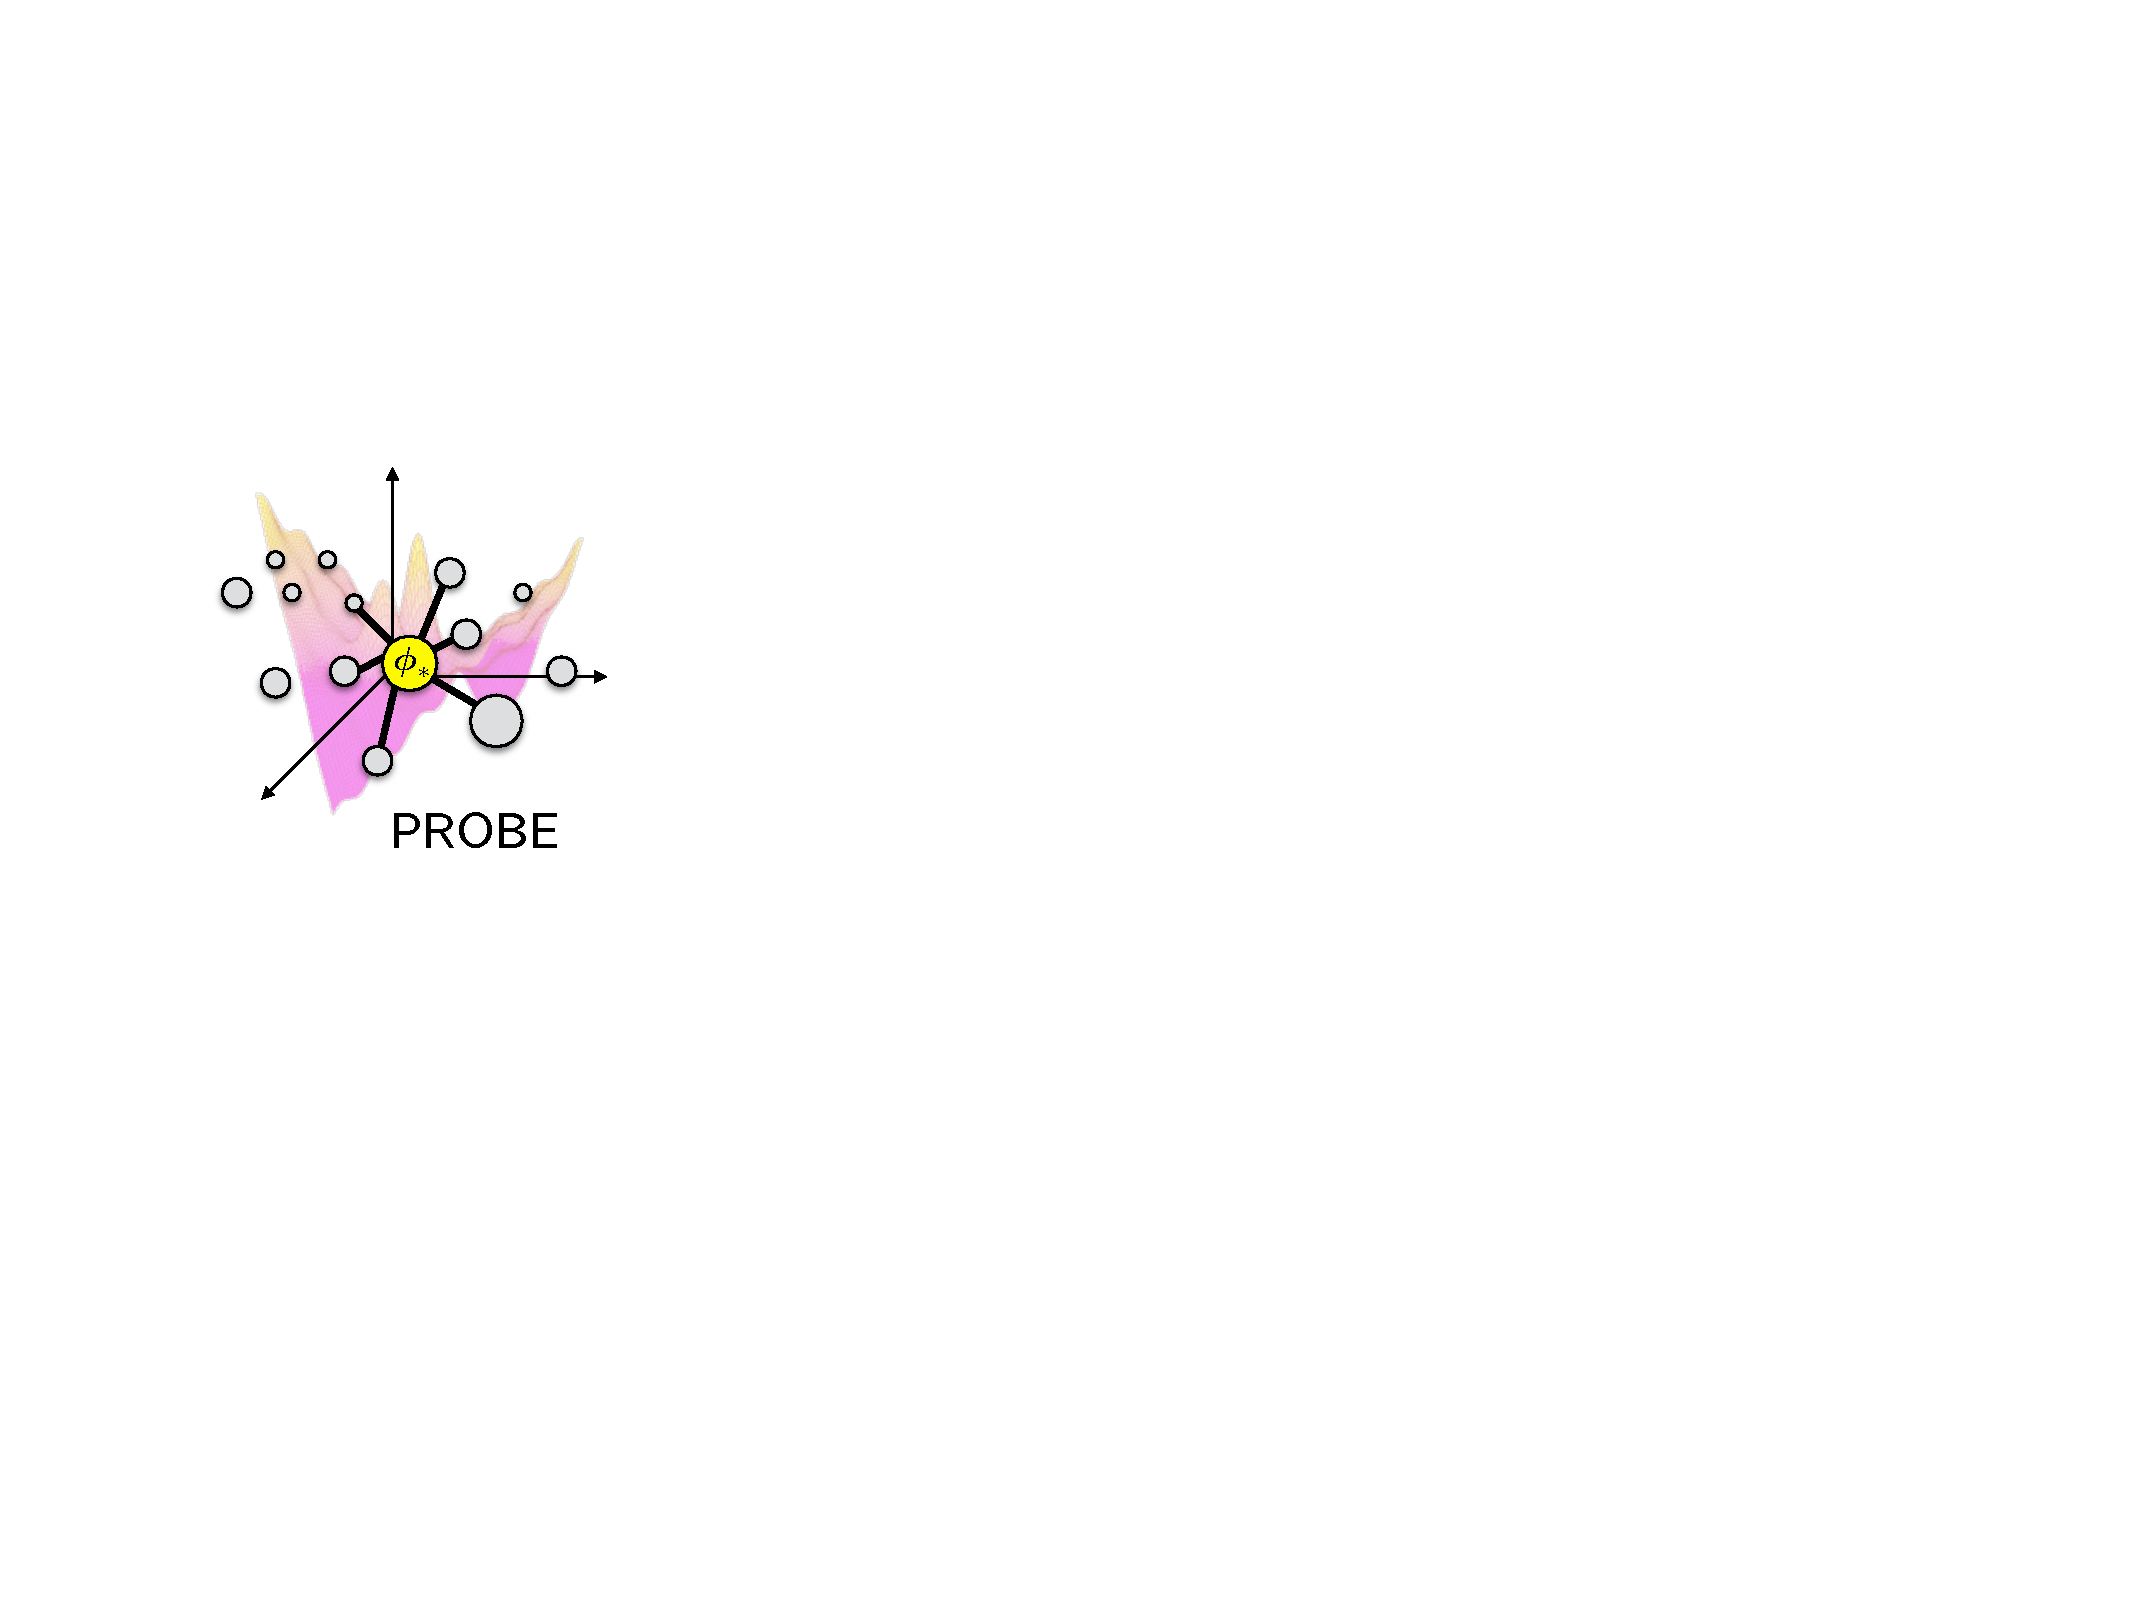
\includegraphics[width=0.8\textwidth]{probe.pdf}
 \caption{PROBE builds a predictive noise model for stereo visual odometry.}
 \label{fig:probe_intro_fig}
\end{figure*}

The first pseudo-sensor we present is a technique we call PRedictive ROBust Estimation, or PROBE. This approach uses non-parametric learning to build a model for anisotropic observation covariances for a stereo visual odometry pipeline. Namely, we apply the method of Generalized Kernel Estimation (GKE) to a Bayesian treatment of covariance estimation. We show that by assuming a particular covariance prior over re-projection errors, we can then naturally derive a robust least squares objective that resembles the widely-used Cauchy loss. The parameters of this robust loss are predicted (hence \textit{predictive} robust estimation) for each error term as a function of a prediction space that we define.

\begin{remark}{Associated Publications}
PROBE was initially published as a simpler non-Bayesian technique that learned isotropic covariances through a k-nearest-neighbours approach (see Appendix \ref{app:appendix_probe_knn} for more details).  The following two publications summarize this initial technique:
\begin{enumerate}
\item \bibentry{2015_Peretroukhin_PROBE}
\item \bibentry{2015_Peretroukhin_Get}.
\end{enumerate}

We significantly extended this technique to full anisotropic covariances and GKE in collaboration with William Vega-Brown at MIT. William was primarily responsible for the mathematical formulation of Generalized Kernels for VO and provided code to perform efficient GKE. I was responsible for the VO formulation, the integration of GKE into the VO pipeline, and all of the experimental work.
\begin{enumerate}[resume]
\item \bibentry{Peretroukhin2016-om}	.
\end{enumerate}
We will present this latter technique in this chapter.
\end{remark}

\section{Motivation}

Robot navigation relies on an accurate quantification of sensor noise or uncertainty in order to produce reliable state estimates.
In practice, this uncertainty is often fixed for a given sensor and experiment, whether by automatic calibration or by manual tuning.
Although a fixed measure of uncertainty may be reasonable in certain static environments, dynamic scenes frequently exhibit many effects that corrupt a portion of the available observations.
For visual sensors, these effects include, for example, self-similar textures, variations in lighting, moving objects, and motion blur. 
Further, there may be useful information available in these observations that would normally be rejected by a fixed-threshold outlier rejection scheme. 
Ideally, we would like to retain some of these observations in our estimator, while still placing more trust in observations that do not suffer from such effects.


\section{Related Work}


There is a large and growing body of work on the problem of deriving accurate,
consistent state estimates from visual data.  Although our approach to noise
modelling is applicable in other domains, for simplicity we focus our attention
on the problem of inferring egomotion from features extracted from sequential
pairs of stereo images. 

Apart from simply rejecting outliers, a number of recent approaches attempt to
select the optimal set of features to produce an accurate localization estimate
from tracked visual features. For example, \citet{Tsotsos2015} amend Random
Sample Consensus (RANSAC) with statistical hypothesis testing to ensure that tracked visual features have normally distributed residuals before including them in
the estimator. Unlike our predictive approach which can adjust covariances from a single observation, their technique requires features to be visible during several consecutive poses. In a different
approach, \Citet{Zhang2015} choose an optimally observable feature subset for a
monocular SLAM pipeline by selecting features with the highest \textit{informativeness} - a measure calculated based on the observability of the SLAM subsystem. Observability, however, is governed by the 3D location of the features, and therefore cannot predict systematic feature degradation due to environmental or sensor-based effects. 


\section{Predictive Robust Estimation for VO}

\begin{figure}
    \centering
      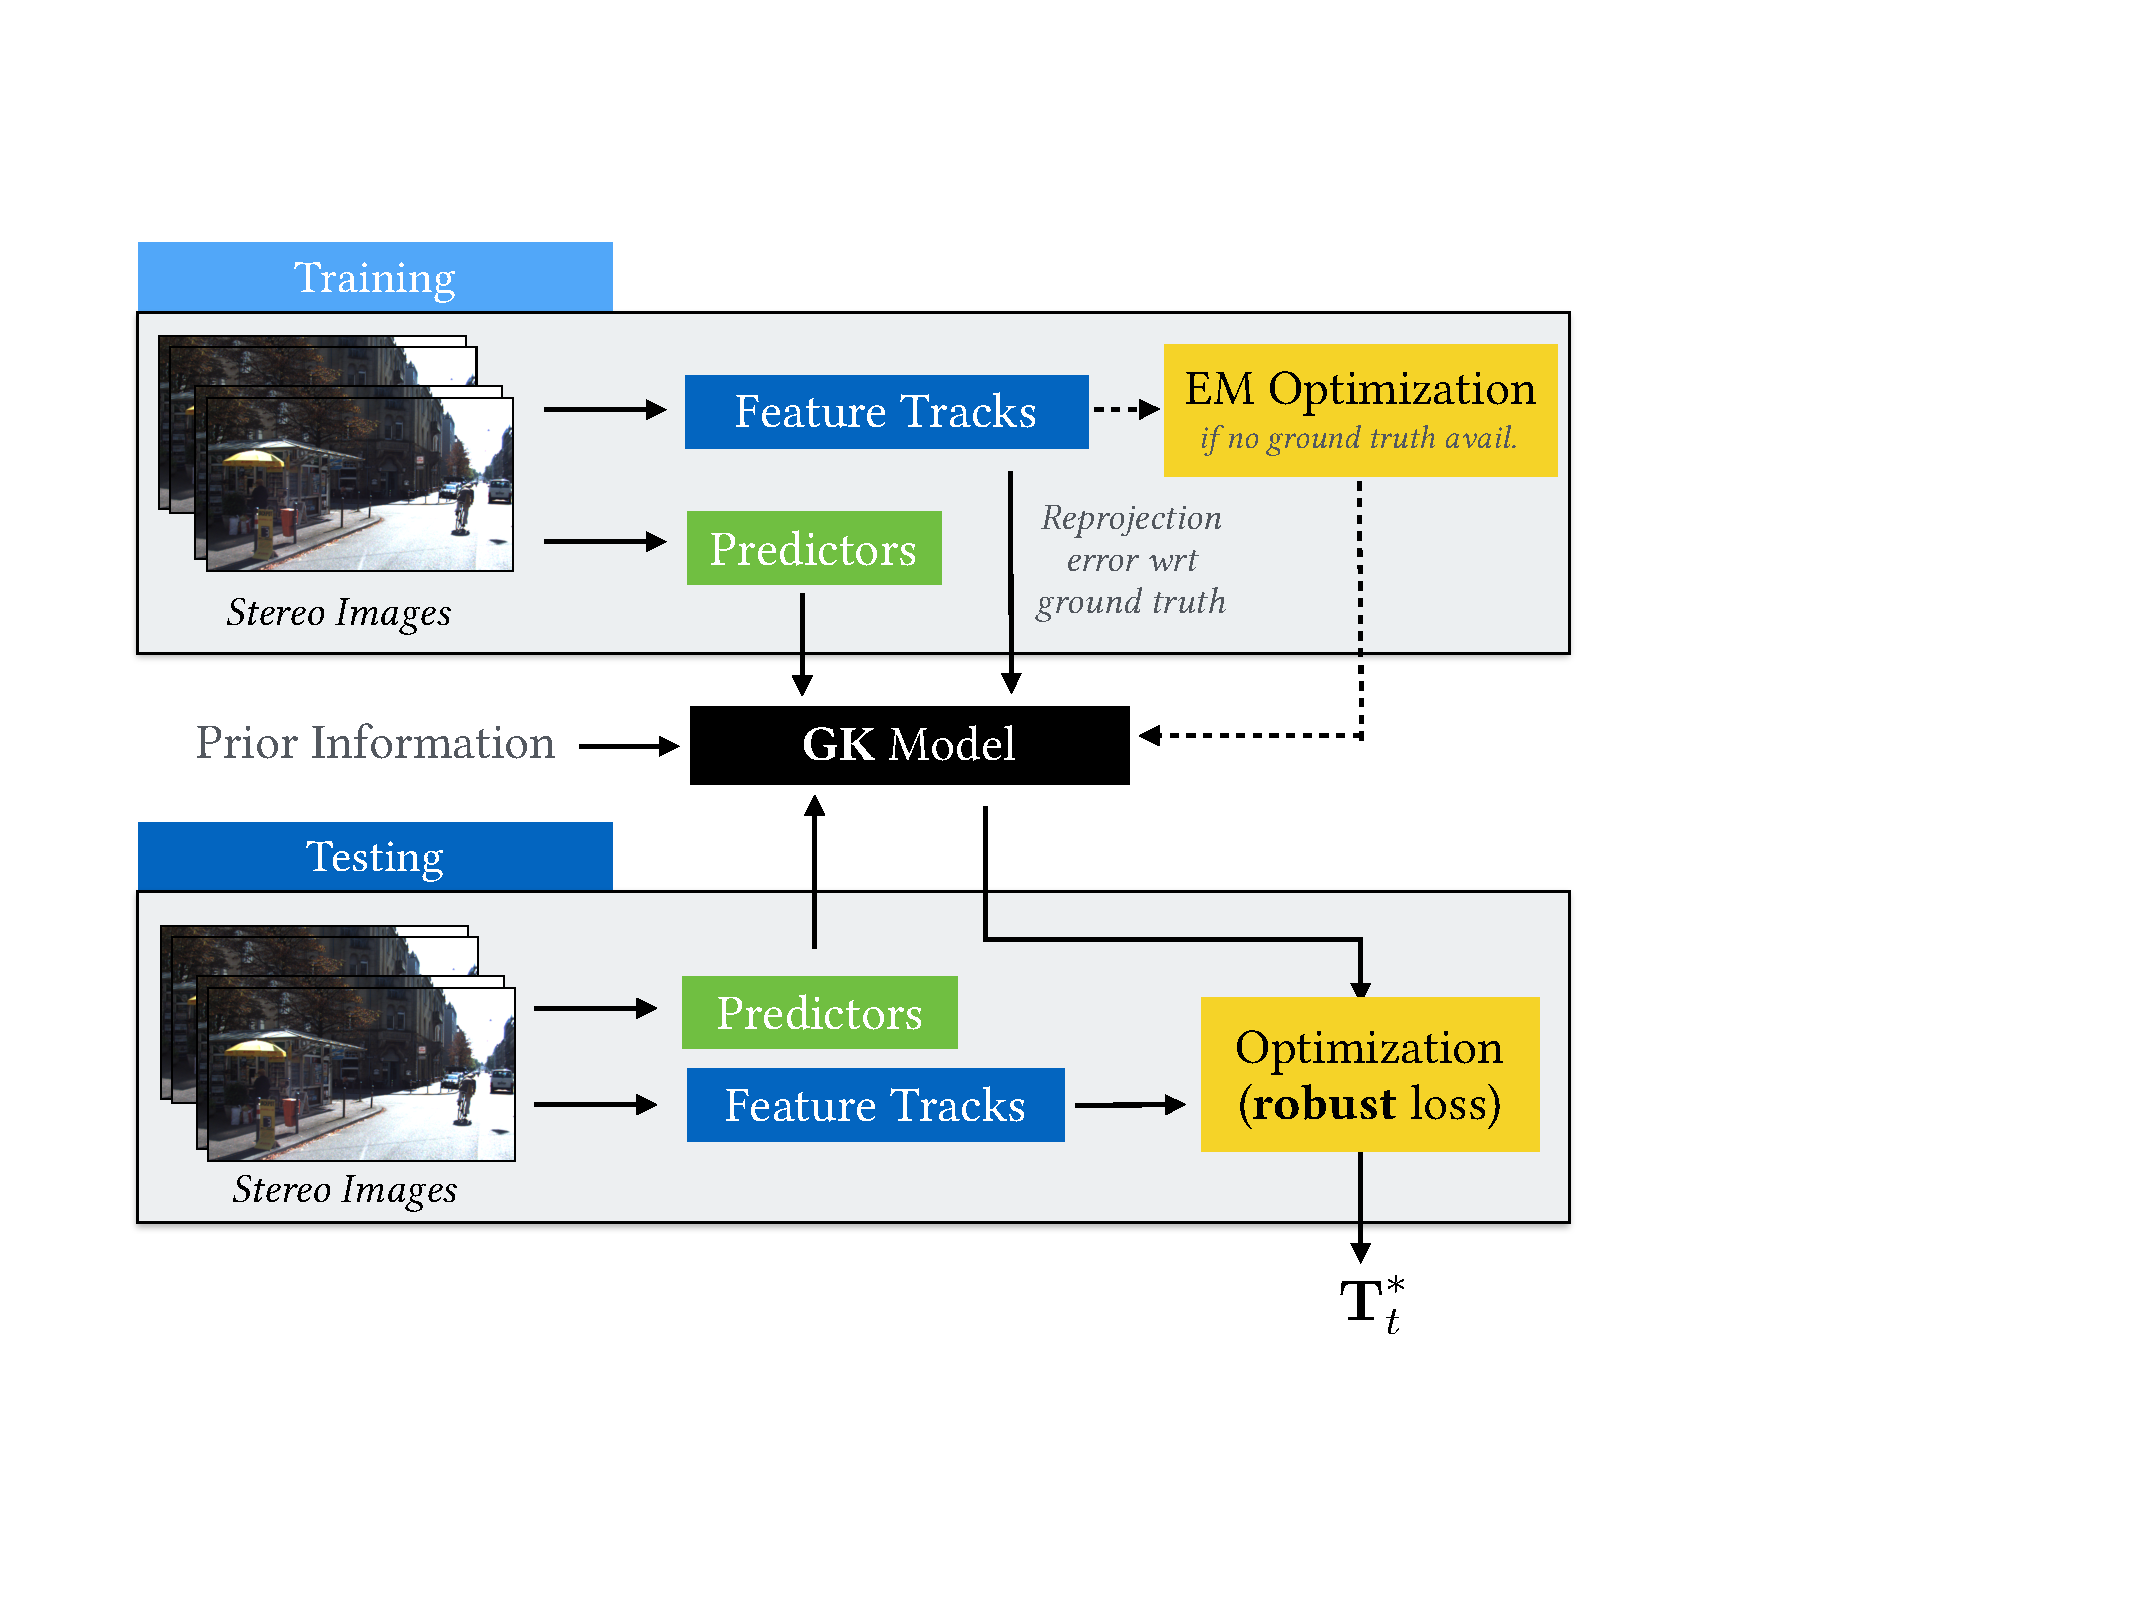
\includegraphics[width=0.65\textwidth]{probe-gk/system_overview}
      \caption{PROBE builds a predictive noise model for stereo visual odometry.}
    \label{fig:probe_gk_system}
\end{figure}

%However, not all features are created equal; most feature-based methods rely on
%random sample consensus algorithms \citep{fischler1981random} to partition the extracted features
%into inliers and outliers, and perform estimation based only on inliers. It is
%common to guard against misclassifying an outlier as an inlier by using robust
%estimation techniques, such as the Cauchy costs employed in
%\citet{kerl2013robust} or the dynamic covariance scaling devised
%by \citet{Burgard:ii}. These approaches, often grouped under the title of M-estimation, aim to maintain a quadratic influence
%of small errors, while reducing the contribution of larger errors. The
%robustness and accuracy of feature-based visual odometry often hinges on the
%tuning of the parameters of inlier selection and robust estimation. Performance
%can vary significantly from one environment to the next, and most algorithms require
%careful tuning to work in a given environment. 

We present a principled, data-driven way to build a noise model
for visual odometry. We leverage recent advances in covariance estimation
\citep{VegaBrown:2013fv} to formulate a predictive robust estimator for a
stereo visual odometry pipeline. We frame the traditional non-linear least
squares optimization problem as a problem of maximum likelihood estimation with
a Gaussian noise model, and infer a distribution over the covariance matrix of
the Gaussian noise from a predictive model learned from training data. This
results in a Student's~$t$ distribution for reprojection error, and naturally yields a
robust nonlinear least-squares optimization problem.  In this way, we can predict,
in a principled manner, how informative each visual feature is with respect to the final state
estimate, which allows our approach to intelligently weight observations to
produce more accurate odometry estimates.  
\subsection{Bayesian Noise Model for Visual Odometry}
We adopt the motion solution for visual odometry based on reprojection errors presented in \Cref{sec:vo_reprojection}. In brief, this technique assumes independent Gaussian errors on stereo reprojections of a landmark from one frame, $\CoordinateFrame{c_0}$ into a subsequent frame, $\CoordinateFrame{c_1}$: 
 \begin{equation}
  \Vector{e}_{i}(\Transform_t) = \Vector{e}_{i,t} = \ImageLandmark{i}{c_1} - \ProjectionFunction( \Transform_t 
    \ProjectionFunction^{-1}( \ImageLandmark{i}{c_0} ) ) \sim 
 \NormalDistribution\left(\Vector 0,  \ImageLandmarkCovariance{i}{t}\right). 
\end{equation}
Maximizing the likelihood of these errors is then equivalent to solving the following weighted non-linear least squares objective for $\Transform_t \in \LieGroupSE{3}$ the rigid-body transform that transforms points in  $\CoordinateFrame{c_0}$ to those in $\CoordinateFrame{c_1}$:
\begin{align}
\label{eq:probe_vo_objective}
  \Transform_t^* &=  \ArgMax{\Transform\in\text{SE}(3)} \prod_{i=1}^{N_t} p(\Vector{e}_{i,t}; \Transform_t,  \ImageLandmarkCovariance{i}{t}) \\
  &= \ArgMin{\Transform\in\text{SE}(3)}\frac{1}{2} \sum_{i=1}^{N_t} 
  \Transpose{\Vector{e}_{i,t}} \ImageLandmarkCovariance{i}{t}^{-1} \Vector{e}_{i,t}.
\end{align}
With PROBE, instead of treating $\ImageLandmarkCovariance{i}{t}$ as fixed, we build a model for it as a function of some useful \textit{predictor}, $\Predictor{i}{t}$, 
\begin{equation}
\ImageLandmarkCovariance{i}{t} = \Covariance(\Predictor{i}{t}).	
\end{equation}
Each predictor can be computed based on the stereo track ($\{\ImageLandmark{i}{c_0}, \ImageLandmark{i}{c_1}\}$) and additional visual\footnote{Including potentially data from all four images in the pair of stereo images.} and inertial cues, allowing us to model effects like motion blur and self-similar textures. Further, instead of treating the covariance as a point function $\Covariance(\Predictor{i}{t})	
$, we instead build a non-parametric model of covariance \textit{density} based on a training dataset, $\mathcal{D}$,
\begin{equation}
	p(\ImageLandmarkCovariance{i}{t}) = p(\Covariance|\mathcal{D}, \Predictor{i}{t}).
\end{equation}
We will seek the transform that then maximizes the posterior predictive distribution of the errors, given this posterior:
\begin{align}
\label{eq:probe_vo_objective}
  \Transform_t^* &=  \ArgMax{\Transform\in\text{SE}(3)} \prod_{i=1}^{N_t} \int p(\Vector{e}_{i,t}; \Transform_t |  \ImageLandmarkCovariance{i}{t}) p(\Covariance|\mathcal{D}, \Predictor{i}{t}) d\Covariance.
\end{align}
Although at first this may seem unwieldy, we present an efficient method for computing the posterior and show that a particular formulation allows it to be marginalized out analytically to arrive at a simple posterior predictive distribution with a straight-forward objective for achieving a maximum likelihood egomotion transform.
\subsection{Generalized Kernels}
To do this, we leverage Generalized Kernel (GK) estimation \citep{Vega-Brown2014-sb}. GK estimation combines the benefits of kernel density estimation with Bayesian inference. The basic idea is as follows. 
Consider a dataset of inputs, $\Vector{x}$, outputs, $\Vector{y}$,  and a dataset of independent observations $\mathcal{D} = \{(\Vector{x}_1, \Vector{y}_1), ..., (\Vector{x}_N, \Vector{y}_N) \}$. We are given a new `test' input $\Vector{x}^*$, and are asked to infer the likelihood of a observing a given output at this input:
\begin{equation}
p(\Vector{y} | 	\Vector{x}^*, \mathcal{D}).
\end{equation}
 If we associate a set of latent parameters, $\GenericParameters$, with each input $\Vector{x}$, and assume a known likelihood function $p(\Vector{y}|\GenericParameters)$, we can infer a distribution over $\GenericParameters$ and then marginalize it out to arrive at the desired likelihood

\begin{equation}
p(\Vector{y} | 	\Vector{x}^*, \mathcal{D}) = \int_{\GenericParameters} \underbrace{p(\Vector{y} | \GenericParameters^*)}_{\text{Known likelihood function}} \underbrace{p(\GenericParameters^* | \Vector{x}^*, \mathcal{D})}_{\text{Parameter posterior}} d\GenericParameters^*.
\end{equation}
This is called the posterior predictive distribution. Using Bayes rule, we can write
\begin{equation}
\label{eq:probe_posterior_bayes_rule}
p(\GenericParameters^* | \Vector{x}^*, \mathcal{D}) \propto \int \left( \prod_{i=1}^N p(\Vector{y}_i | \GenericParameters_i)d\GenericParameters_i \right) p(\GenericParameters_{1:N}, \GenericParameters^*| \Vector{x}^*, \Vector{x}_{1:N})
\end{equation}
The technique of generalized kernels makes the assumption that the parameters $\GenericParameters_{1:N}$ are conditionally independent given the target parameters, $\GenericParameters^*$. This gives the distribution:

\begin{equation}
 p(\GenericParameters_{1:N}, \GenericParameters^*| \Vector{x}^*, \Vector{x}_{1:N}) = \left( \prod_{i=1}^N  p(\GenericParameters_i | \GenericParameters^* \Vector{x}^*, \Vector{x}_i)  \right) p(\GenericParameters^* | \Vector{x}^*), 
\end{equation}
which combined with \Cref{eq:probe_posterior_bayes_rule} results in
\begin{equation}
\label{eq:probe_extended_likelihood}
p(\GenericParameters^* | \Vector{x}^*, \mathcal{D}) \propto \prod_{i=1}^N \underbrace{p(\Vector{y}_i | \GenericParameters^*, \Vector{x}_i, \Vector{x}^*)}_{\text{Extended likelihood}} \underbrace{p(\GenericParameters^*|\Vector{x}^*)}_{\text{Prior}}.
\end{equation}
Now, the pièce de résistance of generalized kernels is that the \textit{extended} likelihood can be written as function of the known likelihood $p(\Vector{y}_i | \GenericParameters_i)$ if we assume it is the maximum entropy distribution whose information divergence from the likelihood is bounded by the metric $\rho(\Vector{x}^*, \Vector{x}_i)$. Specifically, in \cite{Vega-Brown2014-sb}, it is shown that under these assumptions, the extended likelihood must have the form:
\begin{equation}
\label{eq:probe_kernel_likelihood}
p(\Vector{y} | \GenericParameters^*, \Vector{x}, \Vector{x}^*) \propto p(\Vector{y} | \GenericParameters)^{k(\Vector{x}^*, \Vector{x})},
\end{equation}
where $k(\cdot, \cdot)$ is a kernel function\footnote{i.e., $k(\Vector{x}, \Vector{x}) = 1 \forall \Vector{x}$ and $k(\Vector{x}, \Vector{x}') \in [0,1] \forall \Vector{x}, \Vector{x}'$.} that is uniquely defined by $\rho$. The intuition behind this is that we expect the extended likelihood to equal the known likelihood if $\Vector{x}^*$ = $\Vector{x}_i$ (and therefore $\GenericParameters^* = \GenericParameters_i$, resulting in $p(\Vector{y}_i | \GenericParameters^*, \Vector{x}_i, \Vector{x}^*) = p(\Vector{y}_i | \GenericParameters_i)$) and diverge in some smooth way when $\Vector{x}^* \neq \Vector{x}_i$. 
Combining \Cref{eq:probe_extended_likelihood} with \Cref{eq:probe_kernel_likelihood}, we arrive at an expression for the posterior over parameters as 
\begin{equation}
\label{eq:probe_posterior}
p(\GenericParameters | \Vector{x}, \mathcal{D}) \propto \prod_{i=1}^N p(\Vector{y} | \GenericParameters)^{k(\Vector{x}, \Vector{x}_i)} p(\GenericParameters |\Vector{x}),
\end{equation}
which can be evaluated in closed form for appropriate an appropriate likelihood and prior. Namely, for PROBE, we will assume Gaussian likelihoods for the reprojection errors (and therefore the observations $\ImageLandmark{i}{c_1}$), and inverse Wishart priors for covariance matrices (this will result in inverse Wishart posteriors due to conjugacy). The input, $\Vector{x}$, will be the vector of predictors $\Vector{\phi}$.




%Kernel estimation:
%\begin{equation}
%	p(\Vector{\theta} | \mathcal{D}) = \prod_{i=1}^N p (\Vector{y} | \Vector{\theta})^{w_i}
%\end{equation}



\subsection{Generalized Kernels for Visual Odometry}
In
order to exploit conjugacy to a Gaussian noise model, we formulate our prior knowledge
about this function using an inverse Wishart (IW) distribution over positive
definite $d \times d$ matrices (the IW distribution has been used as a prior on covariance matrices in other robotics and computer vision contexts, see for example, \citep{fitzgibbon2007learning}). This distribution is defined by a scale matrix
$\Matrix{\Psi} \in \RealNumbers[d][d]\succ0$ and a scalar quantity called the
degrees of freedom $\nu\in\RealNumbers>d-1$:
\begin{align}
  p\left(\Matrix{R}\right) &= \InverseWishartDistribution
  \left(\Matrix{R}; \Matrix{\Psi}, \nu\right)  \\ 
  &= \frac{\vert\Matrix{\Psi}\vert^{\nu/2}}{2^{\frac{\nu
  d}{2}}\Gamma_d(\frac{\nu}{2})} \vert\Matrix{R}\vert
  ^{-\frac{\nu+d+1}{2}} \exp\left( -\frac{1}{2} \text{tr}\left(\Matrix{\Psi}
  \Matrix{R}^{-1}\right)\right) \nonumber.
\end{align}
We use the scale matrix to encode our prior estimate of the
covariance, and the degrees of freedom to encode our confidence in
that estimate.  Specifically, if we estimate the covariance $\Matrix{R}$
associated with predictor $\Vector{\phi}$ to be $\hat{\Matrix{R}}$ with a
confidence equivalent to seeing $n$ independent samples of the error from
$\NormalDistribution(\Vector{0}, \hat{\Matrix R})$, we would choose
$\nu(\Vector{\phi})=n$ and $\Matrix{\Psi}(\Vector{\phi})=n\hat{\Matrix{R}}$.
Given a sequence of observations and ground truth transformations,
\begin{equation}
\mathcal{D}=\{\mathcal{I}_t,\Transform_t\},\quad t\in[1,N]
\end{equation} 
where
\begin{equation}
 \mathcal{I}_t = \{\ImageLandmark{i}{c_0},
\ImageLandmark{i}{c_1}, \Predictor{i}{t} \} \quad i\in[1,N_t],
\end{equation}
we can use the procedure of generalized kernel estimation as described above to infer a posterior distribution over the
covariance matrix $\TargetImageLandmarkCovariance$ associated with some query
predictor vector $\TargetPredictor$:
\begin{align}
  p(\TargetImageLandmarkCovariance|\mathcal{D}, \TargetPredictor) &\propto
    \prod_{i,t}\mathcal{N}(\Vector{e}_{i,t} \vert \Vector{0},
      \TargetImageLandmarkCovariance)^{k(\TargetPredictor,\Predictor{i}{t})} \nonumber
      \\
      &\qquad\times\text{IW}(\TargetImageLandmarkCovariance;\Matrix{\Psi}(\TargetPredictor),
      \nu(\TargetPredictor)) \\
      &=\text{IW}(\TargetImageLandmarkCovariance;\Matrix{\Psi}_*, \nu_*). 
\end{align}
Here, $\Vector{e}_{i,t}= \ImageLandmark{i}{c_1} - \ProjectionFunction(
\Transform_t \ProjectionFunction^{-1}( \ImageLandmark{i}{c_0} ))$ as before.  
The function $k: \RealNumbers[M]\times\RealNumbers[M]\to[0,1]$ is a kernel
function which measures the similarity of two points in predictor space.
Note also that the posterior parameters $\Matrix{\Psi}_*$ and $\nu_*$ can be
computed in closed form  (see \cite{Vega-Brown2014-sb}) as
\begin{align}
  \Matrix{\Psi}_* &= \Matrix{\Psi}(\TargetPredictor) + 
    \sum_{i,t} k(\TargetPredictor,\Predictor{i}{t}) 
    \Vector{e}_{i,t}\Transpose{\Vector{e}_{i,t}}, \label{eq:compute-psi}\\
  \nu_* &= \nu(\TargetPredictor) + \sum_{i,t}
    k(\TargetPredictor,\Predictor{i}{t}).  \label{eq:compute-nu}
\end{align}
If we marginalize over the covariance matrix, we find that the posterior
predictive distribution is a multivariate Student's~$t$ distribution:
\begin{align}
p(\ImageLandmark{i}{c_1}&|  \Transform_t,\ImageLandmark{i}{c_0}, \mathcal{D},
  \Predictor{i}{t}) \\ &= \int \mathrm{d}\ImageLandmarkCovariance{i}{t}
  \NormalDistribution\left( \Vector{e}_{i,t}; \Vector{0},
    \ImageLandmarkCovariance{i}{t}\right)
  \text{IW}(\ImageLandmarkCovariance{i}{t};\Matrix{\Psi}_*, \nu_*)  \\ &=
  \StudentTDistribution_{\nu_*-d+1}\left(
    \Vector{e}_{i,t}; \Vector{0}, \frac{1}{\nu_*-d+1}\Matrix{\Psi}_*\right) \\ &=
    \frac{\Gamma(\frac{\nu_*+1}{2})}{\Gamma(\frac{\nu_*-d+1}{2})}
    \vert\Matrix{\Psi_*}\vert^{-\frac{1}{2}}\pi^{-\frac{d}{2}} \left(1+
    \Transpose{\Vector{e}_{i,t}} \Matrix{\Psi_*}^{-1} \Vector{e}_{i,t}
  \right)^{-\frac{\nu_*+1}{2}}. 
\end{align}
Given a new landmark and predictor vector, we can infer a noise model by
evaluating \cref{eq:compute-psi,eq:compute-nu}.  In order to accelerate this
computation, it is helpful to choose a kernel function with finite support:
that is, $k(\Vector{\phi},\Vector{\phi}')=0$ if $\Vert\Vector{\phi} -
\Vector{\phi}'\Vert_2 > \gamma$ for some $\gamma$. Then, by indexing our training data in a spatial
index such as a $k$-d tree, we can identify the subset of samples relevant to
evaluating the sums in \cref{eq:compute-psi,eq:compute-nu} in $\mathcal{O}(\log
N + \log N_t)$ time.  \Cref{alg:train-ground-truth} describes the procedure for
building this model. 

\begin{algorithm}
  \caption{Build the covariance model given a sequence of observations, $\mathcal{D}$.}
  \label{alg:train-ground-truth}
  \begin{algorithmic}
    \Function{BuildCovarianceModel}{$\mathcal{D}$}
      \State Initialize an empty spatial index $\mathcal{M}$
      \ForAll{$\mathcal{I}_t,\Transform_t$ in $\mathcal{D}$}
        \ForAll{$\{\ImageLandmark{i}{c_0}, \ImageLandmark{i}{c_1},
          \Predictor{i}{c_0} \}$ in $\mathcal{I}_t$}
          \State $\Vector{e}_{i,t} = \ImageLandmark{i}{c_1} -
            \ProjectionFunction( \Transform_t \ProjectionFunction^{-1}(
            \ImageLandmark{i}{c_0} ))$
            \State Insert $\Predictor{i}{t}$ into $\mathcal{M}$ and store
              $\Vector{e}_{i,t}$ at its location
        \EndFor
      \EndFor
      \State\Return $\mathcal{M}$
    \EndFunction
  \end{algorithmic}
\end{algorithm}

Once we have inferred a noise model for each landmark in a new image pair, the
maximum likelihood optimization problem is given by 
\begin{equation}
  \Transform_t^* = \ArgMin{\Transform_t\in\text{SE}(3)}\sum_{i=1}^{N_t} 
  (\nu_{i,t}+1)\log \left(1+ \Transpose{\Vector{e}_{i,t}}
  \Matrix{\Psi}_{i,t}^{-1} \Vector{e}_{i,t} \right).\label{eq:robust-loss}
\end{equation}
The final optimization problem thus emerges as a nonlinear least squares problem with a rescaled Cauchy-like loss
function, with error term $\Transpose{\Vector{e}_{i,t}}
(\frac{1}{\nu_{i,t}+1}\Matrix{\Psi}_{i,t})^{-1} \Vector{e}_{i,t}$ and outlier
scale $\nu_{i,t}+1$.  This is a common robust loss function which is
approximately quadratic in the reprojection error for
$\Transpose{\Vector{e}_{i,t}} \Matrix{\Psi}_{i,t}^{-1} \Vector{e}_{i,t} \ll
\nu_{i,t}+1$, but grows only logarithmically for $\Transpose{\Vector{e}_{i,t}}
\Matrix{\Psi}_{i,t}^{-1} \Vector{e}_{i,t} \gg \nu_{i,t}+1$.  It follows that in
the limit of large $\nu_{i,t}$---in regions of predictor space where there are
many relevant samples---our optimization problem becomes the original
least-squares optimization problem.

Solving nonlinear optimization problems with the form of  \Cref{eq:robust-loss}
is a well-studied and well-understood task, and software packages to
perform this computation are readily available. 
% TODO: summarize implementation details: how we perform the optimization
\Cref{alg:compute-transform} describes the procedure for computing the transform
between a new image pair, treating the optimization of \Cref{eq:robust-loss} as
a subroutine.

\begin{algorithm}
  \caption{Compute the transform between two images, given a set, $\mathcal{I}_t$,
    of landmarks and predictors extracted from an image pair and a covariance
    model $\mathcal{M}$. }
  \label{alg:compute-transform}
  \begin{algorithmic}
    \Function{ComputeTransform}{$\mathcal{I}_t$, $\mathcal{M}$}
      \ForAll{$\{\ImageLandmark{i}{c_0}, \ImageLandmark{i}{c_1},
      \Predictor{i}{c_0} \}$ in $\mathcal{I}_t$}
        \State $\Matrix{\Psi}, \nu\gets$ \Call{InferNoiseModel} {$\mathcal{M}$, $
          \Predictor{i}{t}$}
        \State $g(\Transform) = \ImageLandmark{i}{c_1} -
          \ProjectionFunction( \Transform\ProjectionFunction^{-1}(
          \ImageLandmark{i}{c_0} ))$
        \State $\mathcal{L} \gets \mathcal{L} +
        (\nu+1)\log\left(1 + \Transpose{g(\Transform)}
          \Matrix{\Psi}^{-1}
        g(\Transform)\right)$
      \EndFor
      \State \Return $\ArgMin{\Transform\in\text{SE}(3)}\mathcal{L}(\Transform)$
    \EndFunction
    \Function{InferNoiseModel}{$\mathcal{M}$, $\TargetPredictor$}
      \State $\textsc{neighbors}\gets$ \Call{GetNeighbors}{$\mathcal{M},
          \TargetPredictor, \rho$} \Comment{$\rho$ is the radius of support of kernel $k$}
      \State $\Matrix{\Psi}_* \gets \Matrix{\Psi}(\TargetPredictor)$ \State
      $\nu_* \gets \nu(\TargetPredictor)$
      \For{$(\Predictor{i}{t},\Vector{e}_{i,t})$ in $\textsc{Neighbors}$}
        \State $\Matrix{\Psi}_* \gets \Matrix{\Psi}_* + k(\TargetPredictor,
          \Predictor{i}{t}) \Vector{e}_{i,t}\Transpose{\Vector{e}_{i,t}}$
        \State $\nu_* \gets \nu_* + k(\TargetPredictor, \Predictor{i}{t})$
      \EndFor
    \State \Return $\Matrix{\Psi}_*, \nu_*$
    \EndFunction
  \end{algorithmic}
\end{algorithm}

We observe that \Cref{alg:compute-transform} is predictively robust, in the
sense that it uses past experiences not just to predict the reliability of a
given image landmark, but also to introspect and estimate its own knowledge of
that reliability.  Landmarks which are not known to be reliable are trusted 
less than landmarks which look like those which have been observed previously, where ``looks like'' is defined by our prediction space and choice of kernel. 

\subsection{Inference without ground truth}

\Cref{alg:train-ground-truth} requires access to the true transform between
training image pairs.  In practice, such ground truth data may be difficult
to obtain.  In these cases, we can instead formulate a likelihood model $p(\mathcal{D}' \vert
\Transform_1, \dots, \Transform_t)$, where $\mathcal{D}' = \{\mathcal{I}_t\}$ is a dataset consisting only of
landmarks and predictors for each training image pair. We can construct a model
for future queries by inferring the most likely sequence of transforms for our
training images.  The likelihood has the following factorized form:
\begin{equation}
  p(\mathcal{D}' \vert \Transform_{1:T}) \propto \int \prod_{i,t}
  \mathrm{d}\ImageLandmarkCovariance{i}{t}\,
  p(\ImageLandmark{i}{c_1} \vert \ImageLandmark{i}{c_0}, 
    \Transform_t, \ImageLandmarkCovariance{i}{t}) p(\ImageLandmarkCovariance{i}{t}\vert \Predictor{i}{t},
    \mathcal{D}, \Transform_{1:T}).
\end{equation}
We cannot easily maximize this likelihood, since marginalizing over the
noise covariances removes the independence of the transforms between
each image pair. To render the optimization tractable, we follow previous work \citep{VegaBrown:2013fv} and formulate an iterative expectation-maximization (EM)
procedure. Given an estimate $\Transform_{t}^{(n)}$ of the transforms, we can
compute the expected log-likelihood conditioned on our current estimate: 
\begin{equation}
  Q(\Transform_{1:T} \vert \Transform_{1:T}^{(n)}) = 
    \int \left(\prod_{i,t}\mathrm{d}\ImageLandmarkCovariance{i}{t}
      \,p(\ImageLandmarkCovariance{i}{t} | \mathcal{D}_{\setminus
        i,t},
      \Transform_{1:T}^{(n)})\right) \log \prod_{i,t} p(\ImageLandmark{i}{c_1} \vert
      \ImageLandmark{i}{c_0}, \Transform_t,
      \ImageLandmarkCovariance{i}{t}).
\end{equation}
This has the effect of rendering the likelihood of each transform to be
estimated independently.  Moreover, the expected log-likelihood can be
evaluated in closed form:
\begin{align}
  Q(\Transform_{1:T} | \Transform_{1:T}^{(n)}) \cong -\frac{1}{2}\sum_{t=1}^T
  \sum_{i=1}^{N_t} \Transpose{\Vector{e}_{i,t}}
  \left(\frac{1}{\nu_{i,t}^{(n)}}\Matrix{\Psi}_{i,t}^{(n)}\right)^{-1}
  \Vector{e}_{i,t}.
\end{align}
The symbol $\cong$ is used to indicate equality up to an additive constant. We can iteratively refine our estimate by maximizing the expected
log-likelihood
\begin{equation}
  \Transform_{1:T}^{(n+1)} = 
    \ArgMax {\Transform_{1:T}\in\text{SE}(3)^T}
    Q(\Transform_{1:T} \vert \Transform_{1:T}^{(n)}).
\end{equation}
Due to the additive structure of $Q(\Transform_{1:T} \vert
\Transform_{1:T}^{(n)})$, this takes the form of $T$ separate nonlinear least-squares optimizations:  
\begin{equation}
\label{eq:Qargmin}
  \Transform_{t}^{(n+1)} = 
    \ArgMin {\Transform_{t}\in\text{SE}(3)}
  \sum_{i=1}^{N_t} \Transpose{\Vector{e}_{i,t}}
  \left(\frac{1}{\nu_{i,t}^{(n)}}\Matrix{\Psi}_{i,t}^{(n)}\right)^{-1}
  \Vector{e}_{i,t}.
\end{equation}
 \Cref{alg:train-em} describes the process of training a model without
ground truth. We refer to this process as PROBE-GK-EM, and distinguish it from
PROBE-GK-GT (Ground Truth). We note that the sequence of estimated transforms,
$\Transform_{1:T}^{(n)}$, is guaranteed to converge to a local maxima of the
likelihood function \citep{dempster1977maximum}. It is also possible to use a robust loss function (\Cref{eq:robust-loss}) in place of \Cref{eq:Qargmin} during EM training. Although not formally motivated by the derivation  above, this approach often leads to lower test errors in practice. Characterizing when and why this robust learning process outperforms its non-robust alternative is outside the scope of this dissertation.

\begin{algorithm}
  \caption{Build the covariance model without ground truth given a sequence of observations, $\mathcal{D'}$, and an initial odometry estimate $\Transform_{1:T}^{(0)}$.}
  \label{alg:train-em}
  \begin{algorithmic}
    \Function{BuildCovarianceModel}{$\mathcal{D'}$, $\Transform_{1:T}^{(0)}$}
      \State Initialize an empty spatial index $\mathcal{M}$
      \ForAll{$\mathcal{I}_t$ in $\mathcal{D'}$}
        \ForAll{$\{\ImageLandmark{i}{c_0}, \ImageLandmark{i}{c_1},
        \Predictor{i}{t} \}$ in $\mathcal{I}_t$}
          \State $\Vector{e}_{i,t} = \ImageLandmark{i}{c_1} -
          \ProjectionFunction( \Transform_t^{(0)} \ProjectionFunction^{-1}(
            \ImageLandmark{i}{c_0} ))$
            \State Insert $\Predictor{i}{t}$ into $\mathcal{M}$ and store
              $\Vector{e}_{i,t}$ at its location
        \EndFor
      \EndFor
      \Repeat
        \ForAll{$\mathcal{I}_t$ in $\mathcal{D'}$}
          \ForAll{$\{\ImageLandmark{i}{c_0}, \ImageLandmark{i}{c_1},
          \Predictor{i}{t} \}$ in $\mathcal{I}_t$}
            \State $\Matrix{\Psi}, \nu\gets$ \Call{InferNoiseModel} {$\mathcal{M}, \Predictor{i}{t}$}
            \State $g(\Transform) = \ImageLandmark{i}{c_1} -
              \ProjectionFunction( \Transform\ProjectionFunction^{-1}(
              \ImageLandmark{i}{c_0} ))$
            \State $\mathcal{L} \gets \mathcal{L} +
              \Transpose{g(\Transform)}
              \left(\frac{1}{\nu}\Matrix{\Psi}\right)^{-1}
              g(\Transform)$
          \EndFor
          \State $\Transform_t \gets \ArgMin{\Transform\in\text{SE}(3)}
            \mathcal{L}(\Transform)$
          \State $\Vector{e}_{i,t} = \ImageLandmark{i}{c_1} -
            \ProjectionFunction( \Transform_t^{(0)} \ProjectionFunction^{-1}(
            \ImageLandmark{i}{c_0} ))$
          \State Update the error stored at $\Predictor{i}{t}$ in $\mathcal{M}$
            to $\Vector{e}_{i,t}$
        \EndFor
      \Until{converged}
      \State\Return $\mathcal{M}$
    \EndFunction
  \end{algorithmic}
\end{algorithm}

\section{Prediction Space} \label{sec:predictors}
A crucial component of our technique is the choice of the vector of predictors $\Vector{\phi}$.
In practice, feature tracking quality is often degraded by a variety of effects such as motion blur, moving objects, and textureless or self-similar image regions.
% Features suffering from such effects are often poorly localized in the image, yet may contain useful information that we would like to retain in our estimator.
% Conversely, we would like to place more trust in features that do not suffer from such effects.
The challenge is in determining predictors that account for such effects without requiring excessive computation.
In our implementation, we use the following predictors, but stress that the choice of predictors can be tailored to suit particular applications and environments:
\begin{itemize}
    \item Angular velocity and linear acceleration magnitudes
    \item Local image entropy
    \item Blur (quantified by the blur metric of \cite{crete2007blur})
    \item Optical flow variance score
    \item Image frequency composition
\end{itemize}
We discuss each of these predictors in turn.


\subsection{Angular velocity and linear acceleration}
While most of the predictors in our system are computed directly from image data, the magnitudes of the angular velocities and linear accelerations reported by an IMU (if available) are in themselves good predictors of image degradation (e.g., image blur) and hence poor feature tracking. 
We do not explicitly correct for bias in linear accelerations because we expect real motion-induced acceleration to trump bias at the timescales of our test trials.  As a result, there is virtually no computational cost involved in incorporating these quantities as predictors.

\subsection{Local image entropy}
Entropy is a statistical measure of randomness that can be used to characterize the texture in an image or patch.
Since the quality of feature detection is strongly influenced by the strength of the texture in the vicinity of the feature point, we expect the entropy of a patch centered on the feature to be a good predictor of its quality.
We evaluate the entropy $S$ in an image patch by sorting pixel intensities into $N$ bins and computing
\begin{equation}
    S = -\sum_{i=1}^N c_i \log_2(c_i),
\end{equation}
where $c_i$ is the number of pixels counted in the $i^\text{th}$ bin.


\subsection{Blur}
Blur can arise from a number of sources including motion, dirty lenses, and sensor defects.
All of these have deleterious effects on feature tracking quality.
To assess the effect of blur in detail, we performed a separate experiment.
We recorded images of 32 interior corners of a standard checkerboard calibration target using a low frame-rate (20 FPS) Skybotix VI-Sensor stereo camera and a high frame-rate (125 FPS) Point Grey Flea3 monocular camera rigidly connected by a bar (\Cref{fig:probe_tricifix}).
Prior to the experiment, we determined the intrinsic and extrinsic calibration parameters of our rig using the \textsc{Kalibr}\footnote{\url{https://github.com/ethz-asl/kalibr}} package \cite{Furgale2013-sl}.
The apparatus underwent both slow and fast translational and rotational motion, which induced different levels of motion blur as quantified by the blur metric proposed by \cite{crete2007blur}.
% The two motion regimes induced different levels of motion blur, which we distinguish by thresholding the blur metric proposed by \cite{Anonymous:Ngi3VEEU}.

\begin{figure}
    \centering
    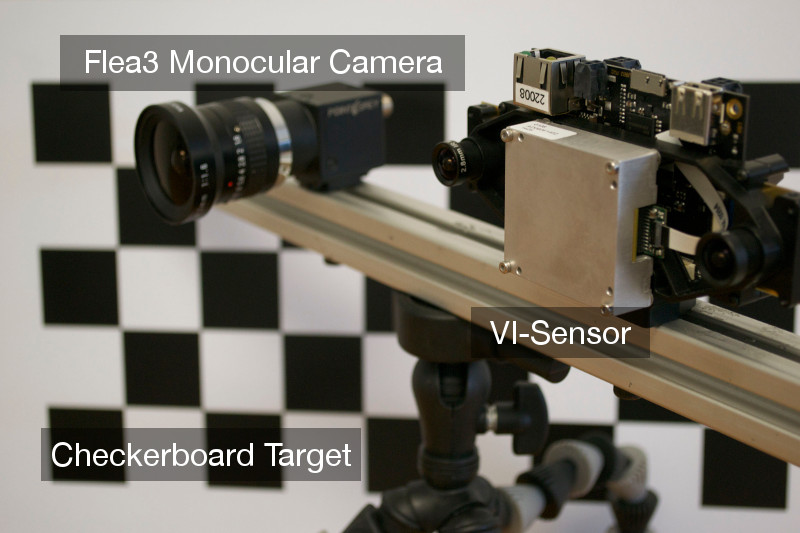
\includegraphics[width=0.5\textwidth]{probe/tricifix2}
    \caption{The Skybotix VI-Sensor, Point Grey Flea3, and checkerboard target used in our motion blur experiments.}
    \label{fig:probe_tricifix}
\end{figure}

%\begin{figure}
%    \centering
%    \includegraphics[width=0.4\textwidth]{figs/blurMetric_short}
%    \caption{Blur metric \cite{Anonymous:Ngi3VEEU} computed for the left camera of the VI-Sensor for the checkerboard dataset. We separate the dataset into regions of high and low blur corresponding to fast and slow motion, respectively.}
%    \label{fig:visensor_blurMetric}
%\end{figure}


\begin{figure}
    \centering
        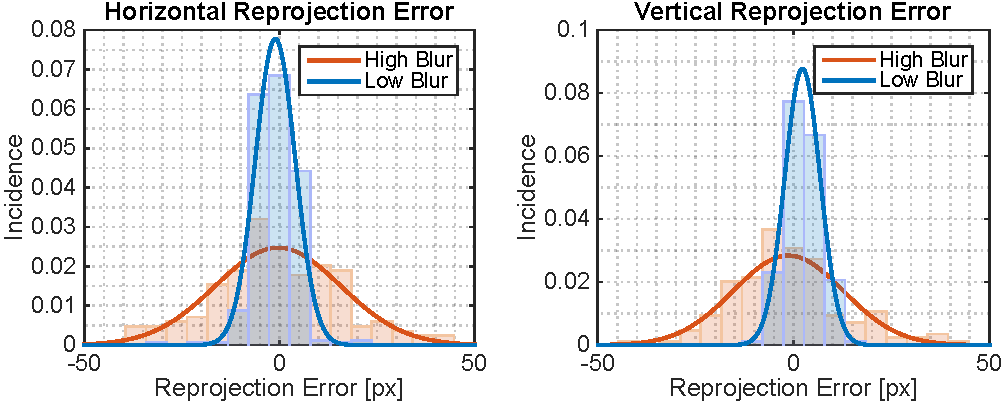
\includegraphics[width=0.85\textwidth]{probe/reprojectionError}
        \label{fig:probe_visensor_reprojectionError}
      \caption{Reprojection error of checkerboard corners triangulated from the VI-Sensor and reprojected into the Flea3.We distinguish between high and low blur by thresholding the blur metric \cite{crete2007blur}.}
\end{figure}

\begin{figure}
    \centering
    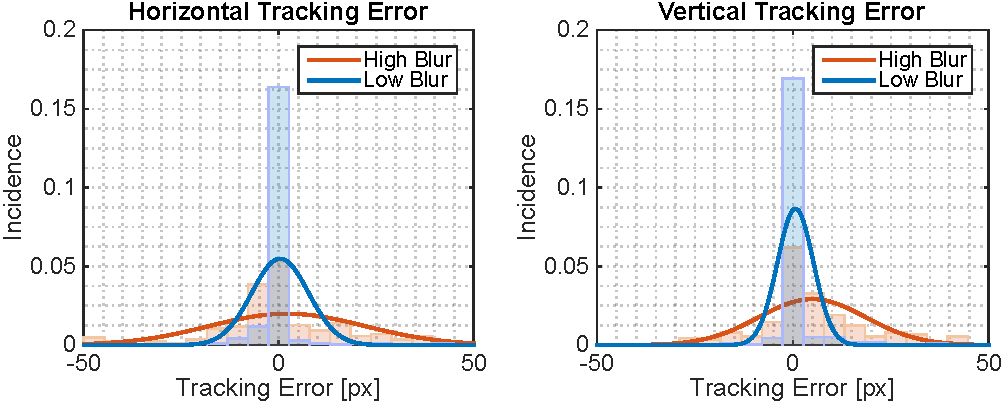
\includegraphics[width=0.85\textwidth]{probe/trackingError}
    \label{fig:probe_visensor_trackingError}
    \caption{Effect of blur on reprojection and tracking error for the slow-then-fast checkerboard dataset. We distinguish between high and low blur by thresholding the blur metric \cite{crete2007blur}. The variance in both errors increases with blur.}
    \label{fig:probe_visensor_histograms}
\end{figure}

We detected checkerboard corners in each camera at synchronized time steps, computed their 3D coordinates in the VI-Sensor frame, then reprojected these 3D coordinates into the Flea3 frame.
We then computed the reprojection error as the distance between the reprojected image coordinates and the true image coordinates in the Flea3 frame.
Since the Flea3 operated at a much higher frame rate than the VI-Sensor, it was less susceptible to motion blur and so we treated its observations as ground truth.
We also computed a tracking error by comparing the image coordinates of checkerboard corners in the left camera of the VI-Sensor computed from both KLT tracking \cite{Lucas:1981} and re-detection.

\Cref{fig:probe_visensor_histograms} shows histograms and fitted normal distributions for both reprojection error and tracking error.
From these distributions we can see that the errors remain approximately zero-mean, but that their variance increases with blur.
This result is compelling evidence that the effect of blur on feature tracking quality can be accounted for by scaling the feature covariance matrix by a function of the blur metric.


\subsection{Optical flow variance}
To detect moving objects, we compute a score for each feature based on the ratio of the variance in optical flow vectors in a small region around the feature to the variance in flow vectors of a larger region.
Intuitively, if the flow variance in the small region differs significantly from that in the larger region, we might expect the feature in question to belong to a moving object, and we would therefore like to trust the feature less.
Since we consider only the variance in optical flow vectors, we expect this predictor to be reasonably invariant to scene geometry.

We compute this optical flow variance score according to
\begin{equation}
    \log \left( \frac{\bar{\sigma}^2_s}{\bar{\sigma}^2_l} \right),
\end{equation}
where $\bar{\sigma}^2_s, \bar{\sigma}^2_l$ are the means of the variance of the vertical and horizontal optical flow vector components in the small and large regions respectively.
\Cref{fig:probe_flow_variance} shows sample results of this scoring procedure for two images in the KITTI dataset.
Our optical flow variance score generally picks out moving objects such as vehicles and cyclists in diverse scenes.

\begin{figure}
    \centering
    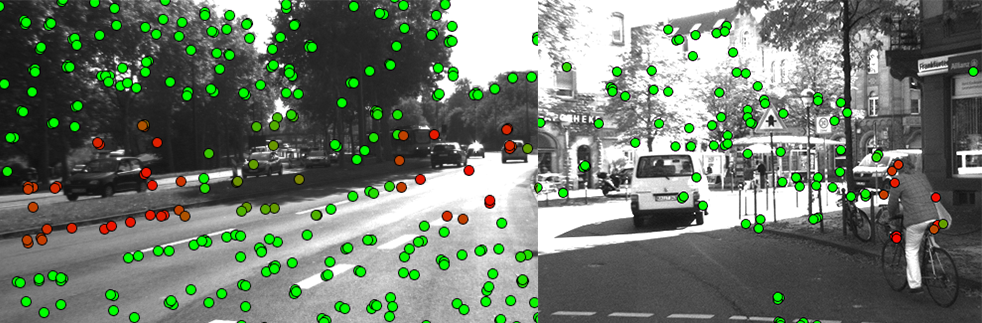
\includegraphics[width=0.8\textwidth]{probe/flowPredictorCombined.png}
    \caption{The optical flow variance predictor can help in detecting moving objects. Red circles correspond to higher values of the optical flow variance score (i.e., features more likely to belong to a moving object).}
    \label{fig:probe_flow_variance}
\end{figure}

\subsection{Image frequency composition}
Reliable feature tracking is often difficult in textureless or self-similar environments due to low feature counts and false matches.
We detect textureless and self-similar image regions by computing the Fast Fourier Transform (FFT) of each image and analyzing its frequency composition.
For each feature, we compute a coefficient for the low- and high-frequency regimes of the FFT.
\Cref{fig:probe_high_frequency} shows the result of the high-frequency version of this predictor on a sample image from the KITTI dataset.
Our high-frequency predictor effectively distinguishes between textureless regions (e.g., shadows and roads) and texture-rich regions (e.g., foliage).


\begin{figure}
    \centering
    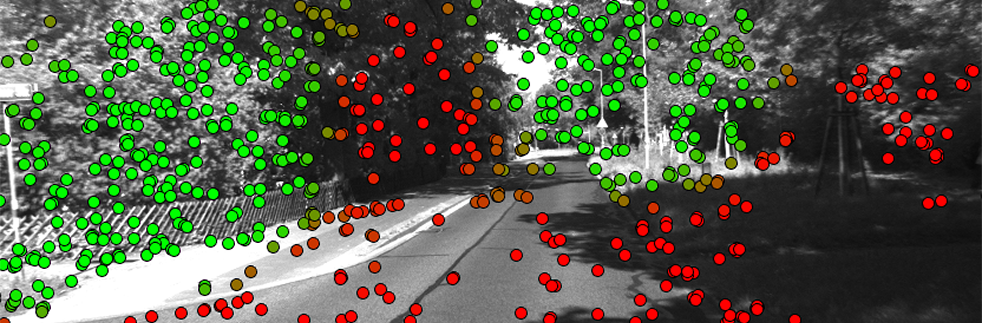
\includegraphics[width=0.8\textwidth]{probe/highFreqPredictor.png}
    \caption{A high-frequency predictor can distinguish between regions of high and low texture such as foliage and shadows. Green indicates higher values.}
    \label{fig:probe_high_frequency}
\end{figure}


\section{Experiments}
To validate PROBE-GK, we used three types of data: synthetic simulations, the
KITTI dataset, and our own experimental data collected at the University of
Toronto. 

\subsection{Simulation}
\subsubsection{Monte-Carlo Verification}
To begin, we verified that PROBE-GK can predict increasingly accurate estimates of the true error covariance as more training data is added. We developed a basic simulation environment consisting of a large amount of point landmarks being observed by a stereo camera. In our simulation, the camera traversed a single step in one direction, and recorded  empirical reprojection errors based on ground truth poses. We simulated additive Gaussian noise on image coordinates, and used Monte Carlo simulations to estimate the true covariances. \Cref{fig:probe_frobNorm} shows the mean Frobenius norm (as defined in \cite{Barfoot2014-ac}) between the covariances estimated by PROBE-GK and the true covariances for a test trial. The mean norm tends to zero as more landmarks are added, indicating that PROBE-GK does learn the correct covariances.


\begin{figure}
    \centering
      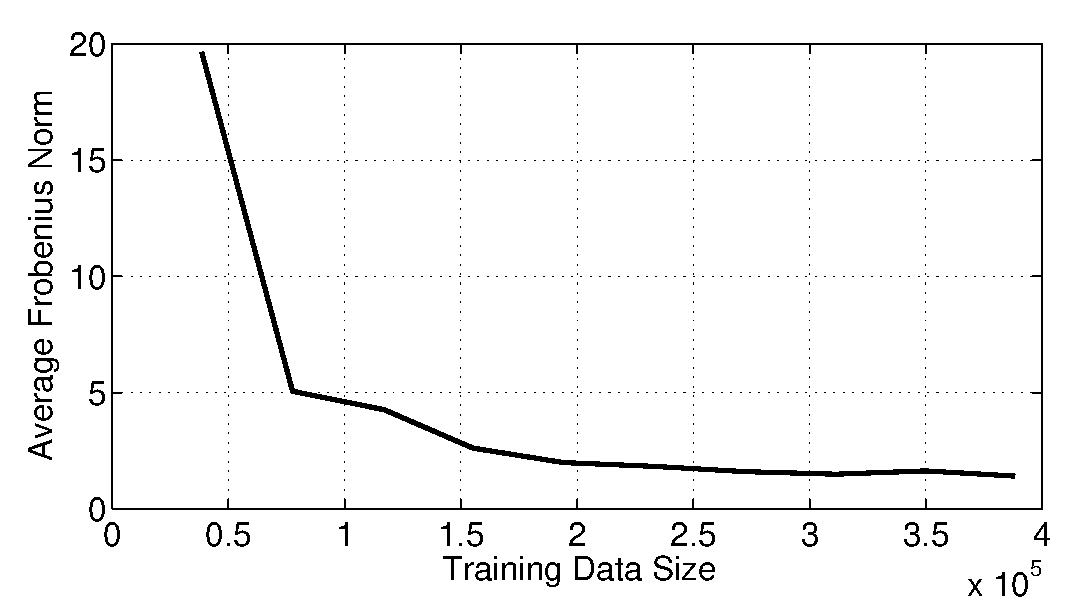
\includegraphics[width=0.45\textwidth]{probe-gk/frobNorm.eps}
     \caption{Mean Frobenius norm of the error between the estimated and true
       noise covariance as a function of training data size. The norm tends to
       zero as training data is added which indicates that PROBE-GK is learning
       the correct covariances.}
    \label{fig:probe_frobNorm}
\end{figure}


\subsubsection{Synthetic}

Next, we formulated a synthetic dataset wherein a stereo camera traverses a circular path observing 2000 randomly distributed point features.
We added Gaussian noise to each of the ideal projected
pixel co-ordinates for visible landmarks at every step. We varied the noise variance as a function of the vertical pixel coordinate of
the feature in image space. In addition, a small subset of the landmarks received an error term drawn from a uniform distribution to simulate the presence of outliers. The prediction space was composed of
the vertical and horizontal pixel locations in each of the stereo cameras.

\begin{figure}
\centering
   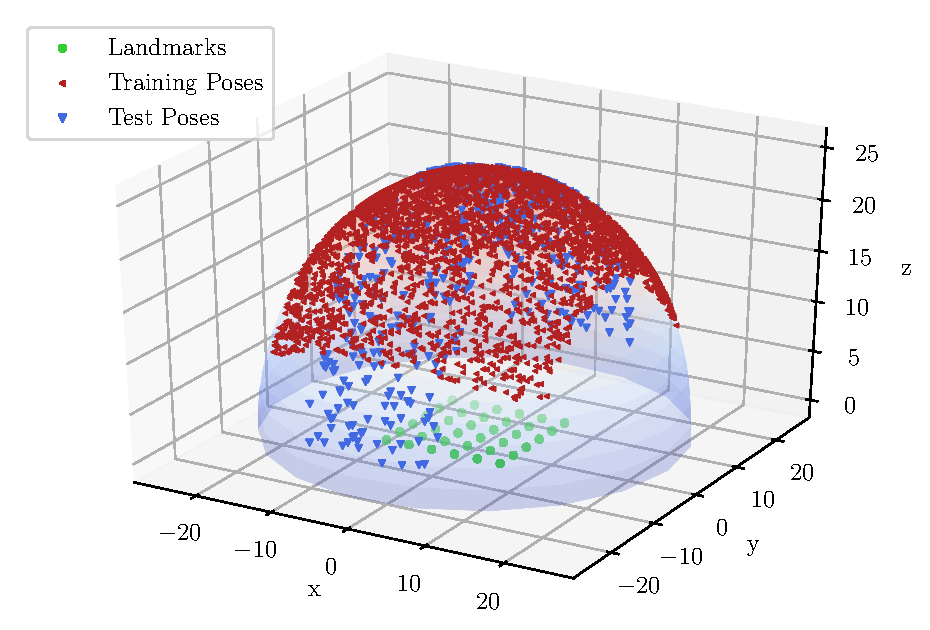
\includegraphics[width=0.5\textwidth]{probe-gk/sim_world.pdf}
   \label{fig:probe_SimWorld} 
\caption{Our synthetic world. A stereo camera rig moves through a world with 2000 point features.}
\end{figure}

We simulated independent training and test traversals, where the camera moved for
30 and 60 seconds respectively (at a forward speed of 3 metres per second for final path
lengths of 90 and 180 meters).  \Cref{fig:probe_sim_comparison} and \Cref{table:probe-gk_armse_errors} document the qualitative and quantitative comparisons of PROBE-GK (trained with and without ground-truth) against two baseline stereo odometry frameworks. Both baseline estimators were implemented based on the reprojection-error-based VO pipeline described in  \Cref{ch:vo}. The first utilized fixed covariances for all reprojection errors, while the second used a modified robust cost (i.e. M-estimation) based on Student's~$t$ weighting, with $\nu = 5$ (as suggested in \cite{kerl2013robust}).  These benchmarks served as baseline estimators (with and without robust costs) that used fixed covariance matrices and did not include a predictive component. 

Using PROBE-GK with ground truth data for training,
we significantly reduced both the translation and rotational Average Root Mean Squared Error (ARMSE)
by approximately 50\%. In our synthetic data, the Expectation Maximization approach was able to achieve nearly identical results to the ground-truth-aided model within 5 iterations.  

\begin{figure}
    \centering
    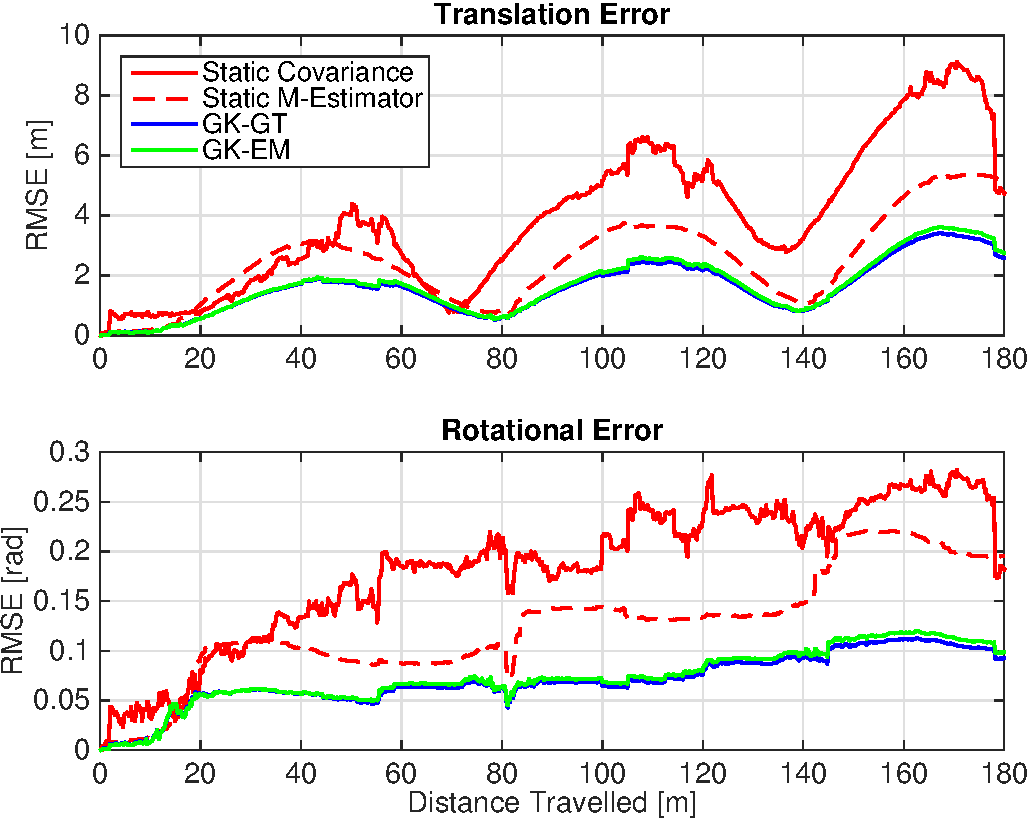
\includegraphics[width=0.75\textwidth]{probe-gk/simComparison_sim_rerun}
    \caption{A comparison of translational and rotational Root Mean Square Error on simulated data
    (RMSE) for four different stereo-visual odometry pipelines: two baseline
    bundle adjustment procedures with and without a robust Student's~$t$ cost with a fixed and
    hand-tuned covariance and degrees of freedom (M-Estimation), a robust bundle
    adjustment with covariances learned from ground truth with
    \cref{alg:train-ground-truth} (GK-GT), and a robust bundle adjustment using
    covariances learned without ground truth using expectation maximization,
    with \cref{alg:train-em} (GK-EM). Note in this experiment, the RMSE curves
    for GK-GT and GK-EM very nearly overlap. The overall translational and
    rotational ARMSE values are shown in Table \ref{table:probe-gk_armse_errors}.} 
    \label{fig:probe_sim_comparison}
\end{figure}

\subsection{KITTI}

\begin{figure}
    \centering
    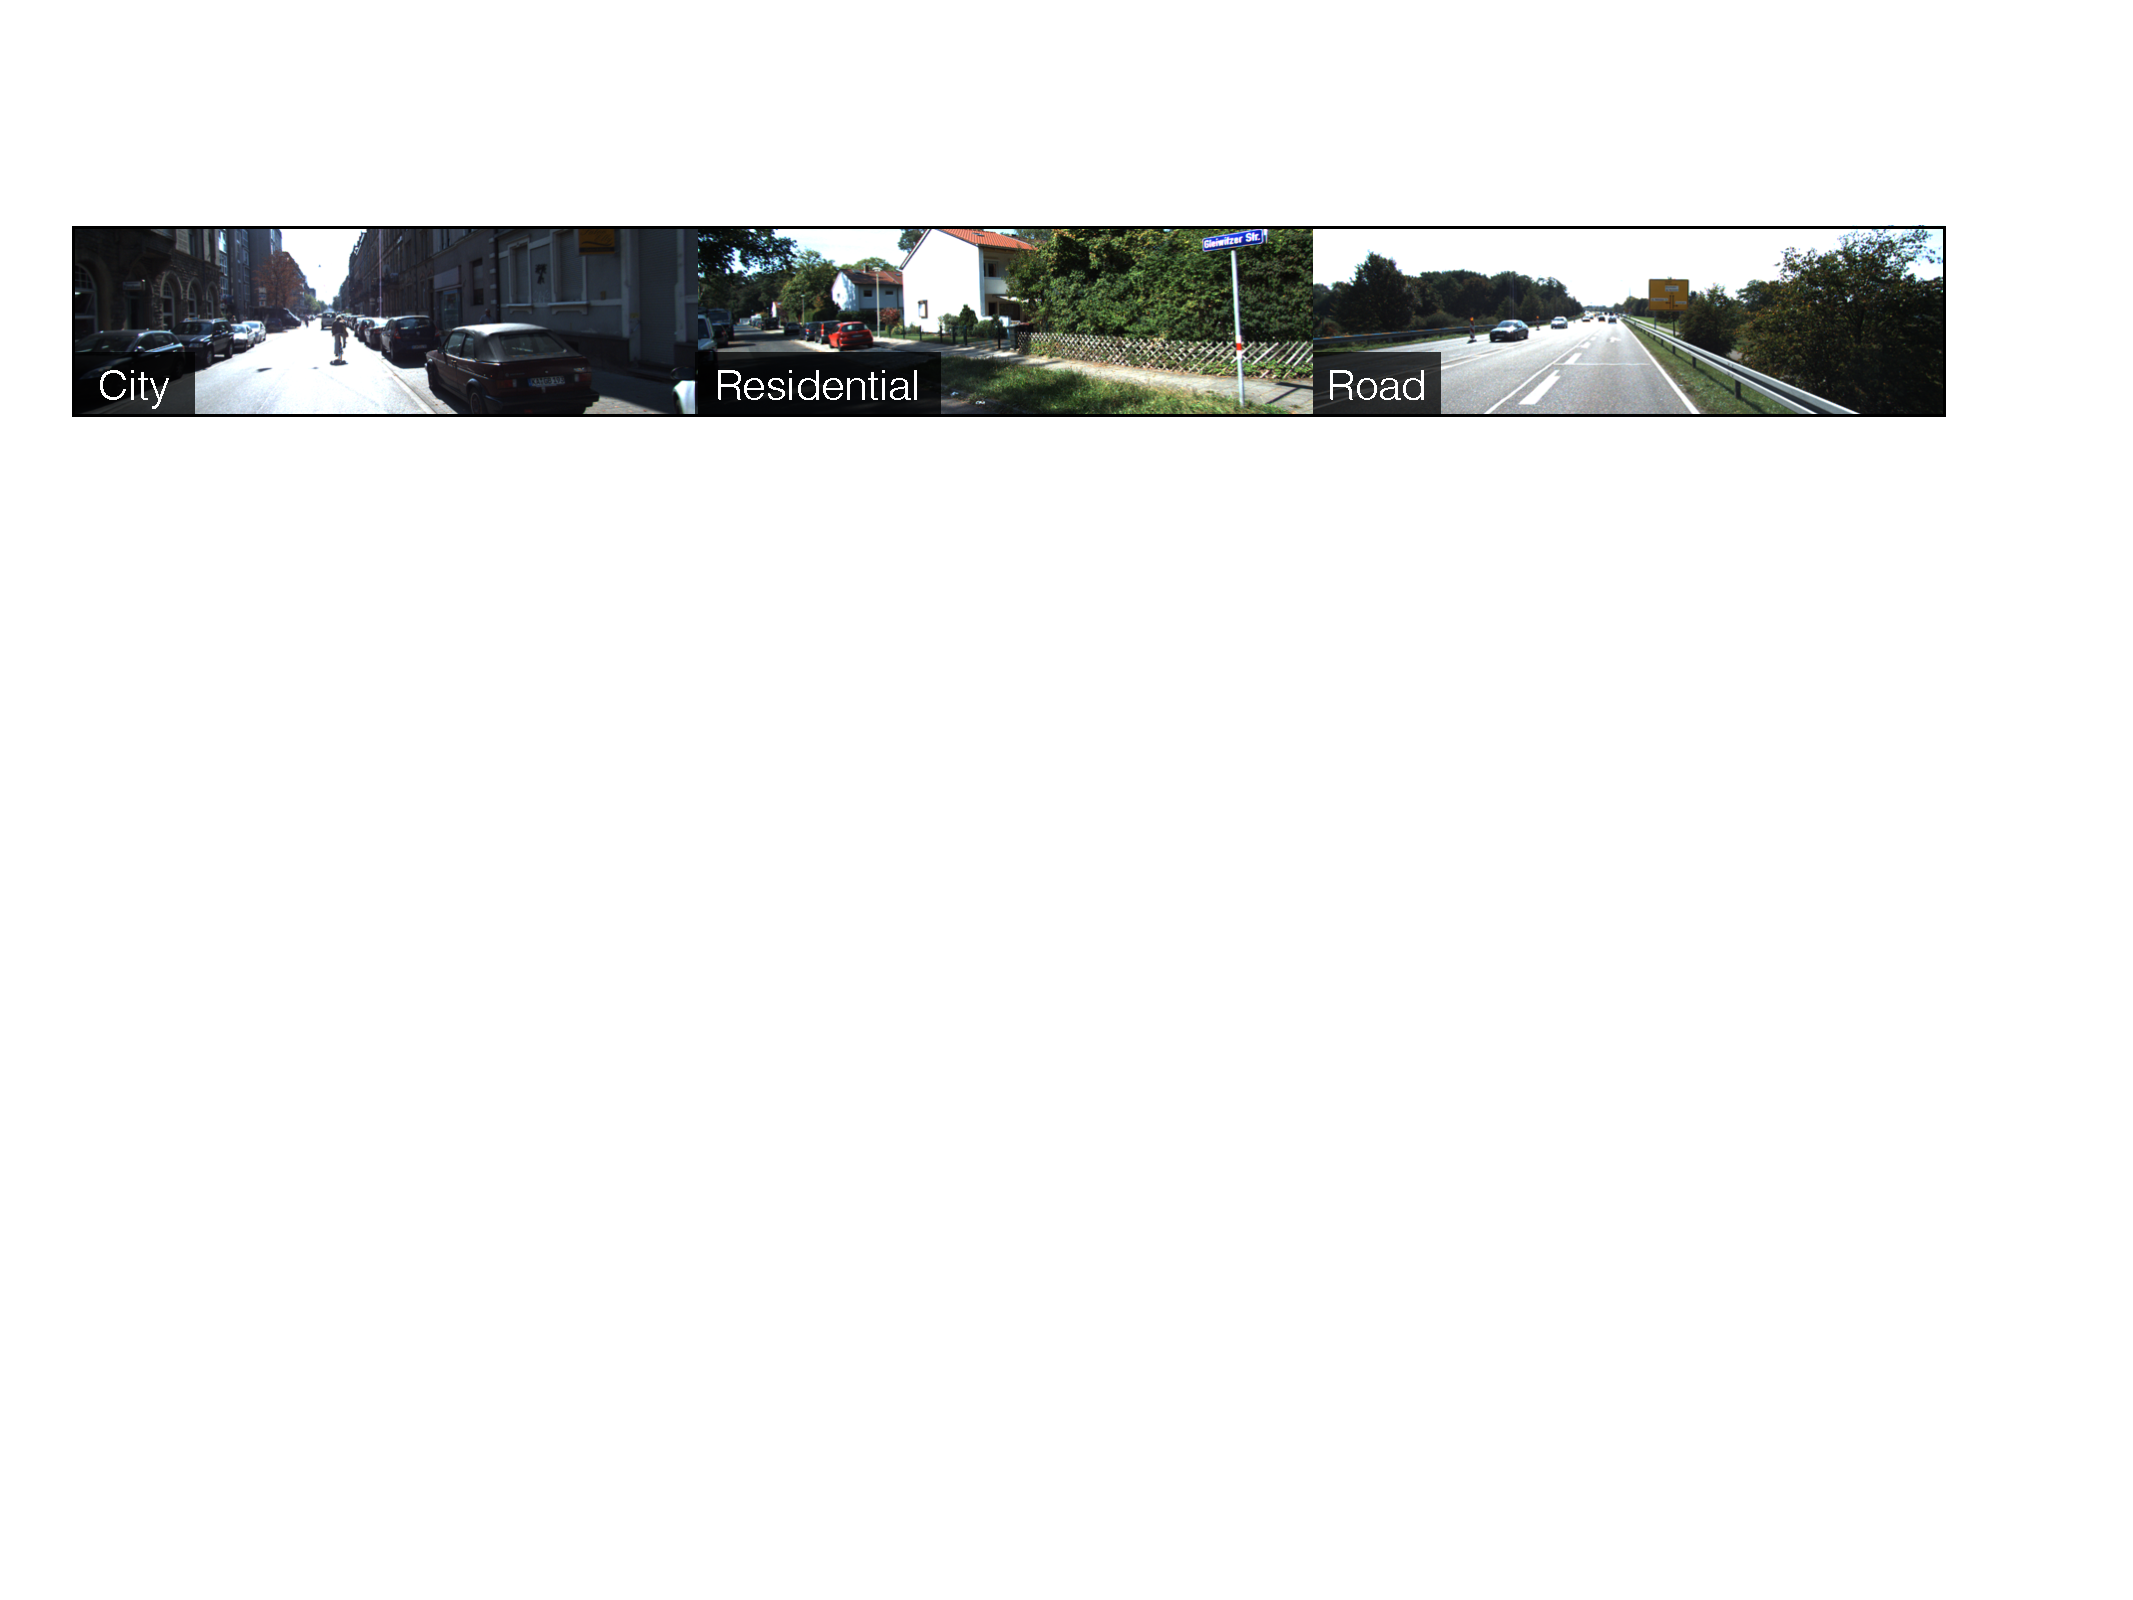
\includegraphics[width=0.98\textwidth]{probe-gk/KittiEnvironments}
    \caption{The KITTI dataset contains three different environments. We
      validate PROBE-GK by training on each type and testing against a baseline
      stereo visual odometry pipeline.}
      \vspace{-0.5em}
    \label{fig:kitti_environments}
\end{figure}

To evaluate PROBE-GK on real environments, we trained and tested several models on
the KITTI Vision Benchmark suite \citep{Geiger2013-ky}, a series of datasets collected by a car outfitted with a number of
sensors driven around different parts of Karlsruhe, Germany. Within the dataset, ground truth pose information is
provided by a high grade inertial navigation unit which also fuses measurements from differential GPS. Raw data
is available for different types of environments through which the car was driving; for our
work, we focused on the city, residential and road categories
(\Cref{fig:kitti_environments}).  From each category, we chose two separate trials for training and testing.


\begin{figure}
	\centering
	 \begin{subfigure}{0.48\textwidth}
	 \includegraphics[width=\textwidth]{probe-gk/{kittiComparison-0011-0009-15-Sep-2015-4way}}
    \caption{City category.}
    \label{fig:probe-gk_kitti_comparison1}
    \end{subfigure}
    ~
    \begin{subfigure}{0.48\textwidth}
    	\includegraphics[width=\textwidth]{probe-gk/{kittiComparison-0035-0036-15-Sep-2015-4way}}
    \caption{Residential category.}
    \label{fig:probe-gk_kitti_comparison2}    \end{subfigure}
    ~
    \begin{subfigure}{0.48\textwidth}
    	\includegraphics[width=\textwidth]{probe-gk/{kittiComparison-0070-0028-15-Sep-2015-4way}}
    \caption{Road category.}
    \vspace{-0.4em}
    \label{fig:probe-gk_kitti_comparison3}    \end{subfigure}

    \caption{RMSE comparison of stereo VO estimators evaluated on data in the KITTI odometry benchmark. See \Cref{table:probe-gk_armse_errors} for a quantitative summary.}
     \label{fig:probe-gk_kitti_comparison_overall}
\end{figure}


\Cref{fig:probe-gk_kitti_comparison1,fig:probe-gk_kitti_comparison2,fig:probe-gk_kitti_comparison3} show
typical results; \Cref{table:probe-gk_armse_errors} presents a quantitative comparison.
PROBE GK-GT produced significant reductions in ARMSE, reducing translational ARMSE by
as much as 80\%. In contrast, GK-EM showed more modest improvements; this is
unlike our synthetic experiments, where both GK-EM and GK-GT achieved similar
performance. We note that although our simulated
data is drawn from a mixture of Gaussian distributions, the underlying
noise distribution for real data may be far more complex. With no ground truth, EM has to jointly optimize the camera poses and sensor uncertainty. It is unclear whether this is feasible in the general case with no ground truth information.

Further, we observe that the performance of PROBE-GK depends on the similarity
of the training data to the final test trials. A characteristic training dataset was important for consistent improvements on test trials.


\subsection{UTIAS}

\begin{table}
\centering
\caption{Comparison of average root mean squared errors (ARMSE) for rotational
  and translational components. Each trial is trained and tested from a
  particular category of raw data from the synthetic and KITTI datasets.}

\resizebox{\columnwidth}{!}{%
\begin{tabular}{l c c c c c c c c c }
 & & \multicolumn{4}{c}{Trans. ARMSE [m]} & \multicolumn{4}{c}{Rot. ARMSE [rad]}  \\  \cline{3-6}  \cline{7-10} \T                                                                                    
 & Length [m] & Fixed Covar. & Static M-Estimator  & GK-GT & GK-EM & Fixed Covar. &  Static M-Estimator  & GK-GT & GK-EM  \\                         
\hline \T
Synthetic & 180 & 3.87 & 2.49 & 1.59 & 1.66 & 0.18 & 0.13 & 0.070 & 0.073 \\                                                                                                                
City & 332.9 & 3.84 & 2.99 & 1.69 & 2.87 & 0.032 & 0.021 & 0.0046 & 0.018 \\ 
Residential & 714.1 & 13.48 & 9.37 & 1.97 & 8.80 & 0.068 & 0.050 & 0.013 & 0.044 \\
Road & 723.8 & 17.69 & 9.38 & 5.24 & 8.87 & 0.060 & 0.027 & 0.015 & 0.024
\\ \hline                                                                                                                
\end{tabular}               \label{table:probe-gk_armse_errors}
}
\end{table}

\begin{figure}
	\centering
	 \begin{subfigure}{0.49\textwidth}
	 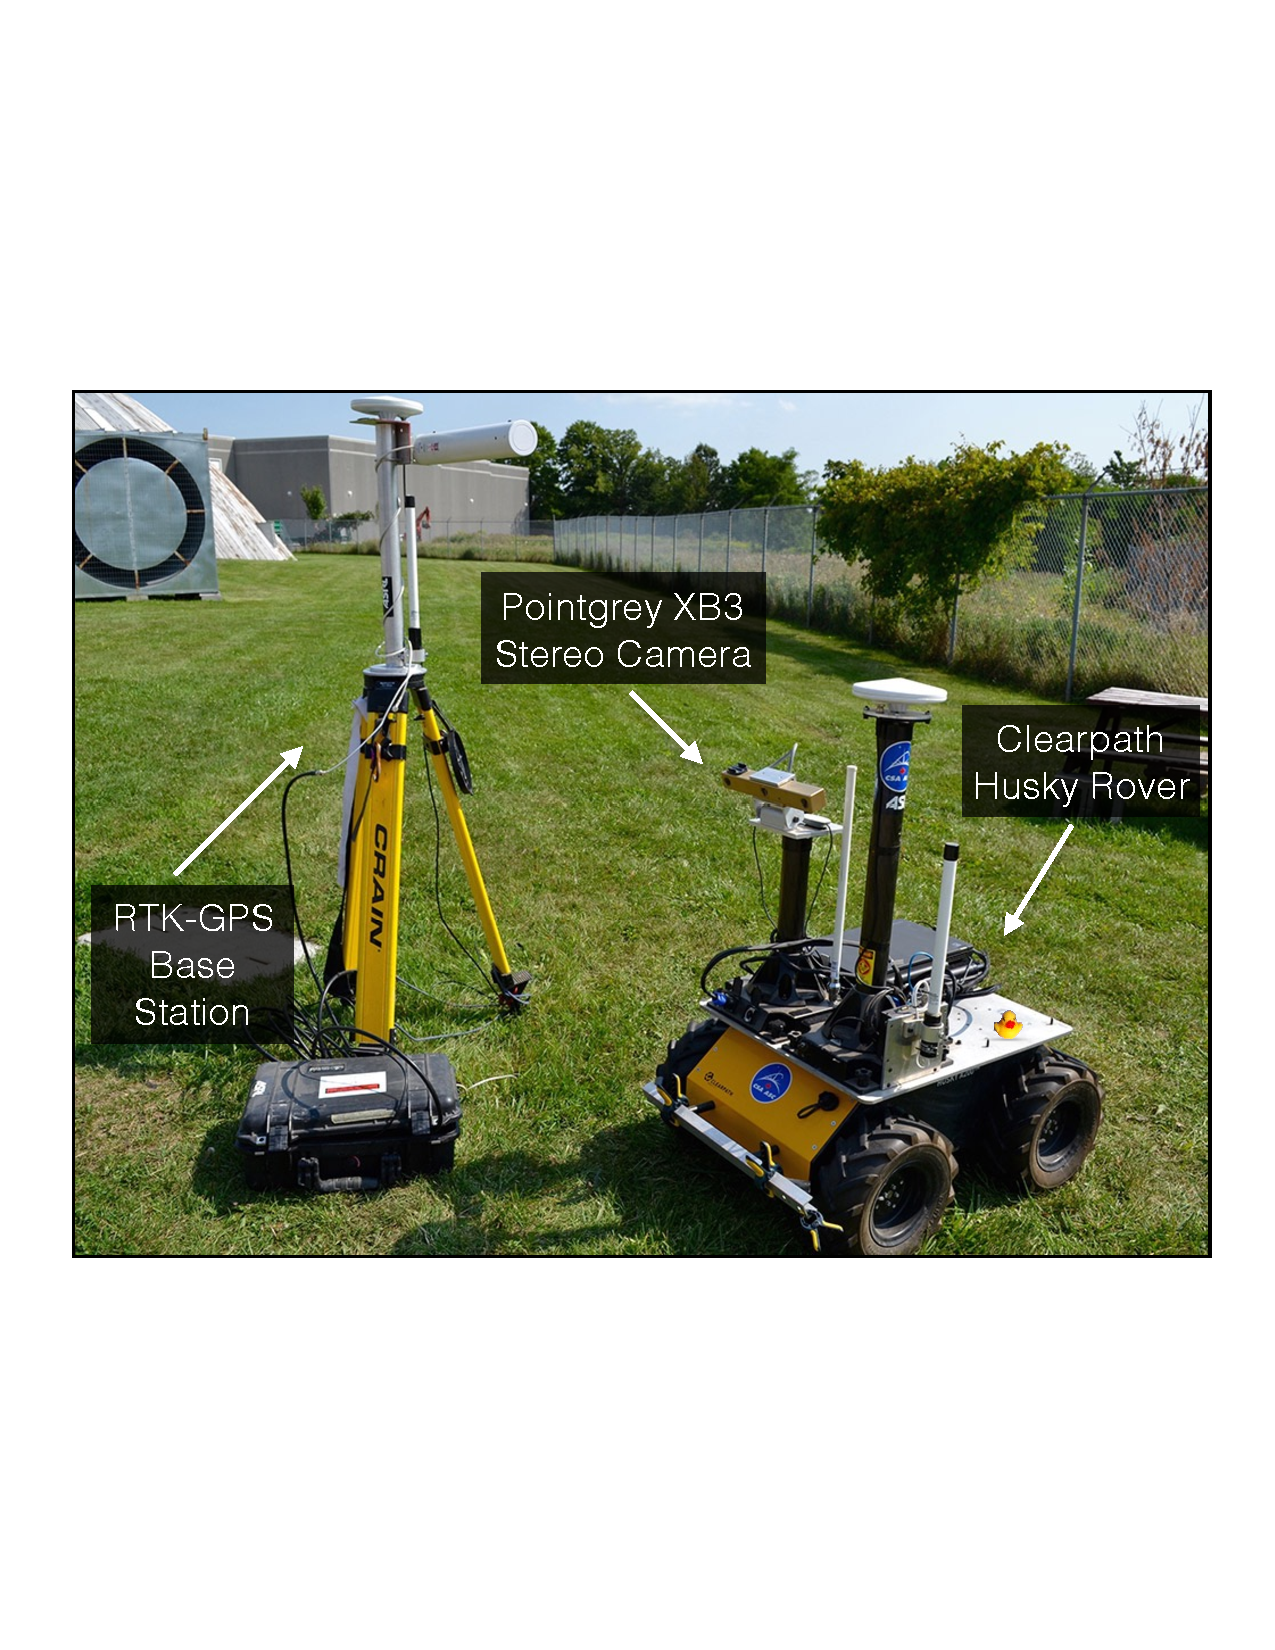
\includegraphics[width=\textwidth]{probe-gk/experiment_wide_border}
    \caption{Our experimental apparatus: a Clearpath Husky rover outfitted with a PointGrey XB3 stereo camera and a differential GPS receiver and base station.}
      \vspace{-0.5em}
   	    \label{fig:probe-gk_experiments}
    \end{subfigure}
    ~
    \begin{subfigure}{0.49\textwidth}
    	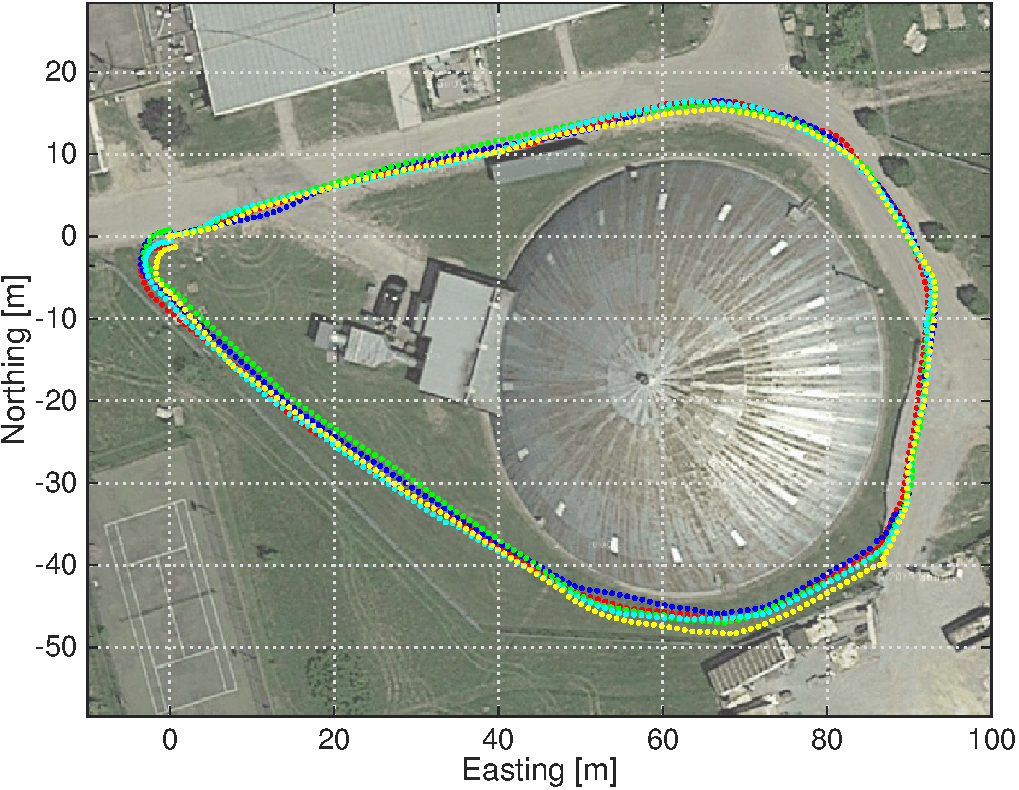
\includegraphics[width=\textwidth]{probe-gk/xb3_rtk_fig}
    \caption{GPS ground truth for 5 experimental trials collected
      near the UTIAS Mars Dome. Each trial is approximately 250 m long.}
      \vspace{-0.5em}
    \label{fig:probe-gk_experiment_groundtruth}   \end{subfigure}
    \caption{Our experimental setup.}
     \label{fig:probe-gk_experiments_overall}
\end{figure}

\begin{figure}
    \centering
    \includegraphics[width=0.75\textwidth]{probe-gk/{trainingStats}}
    \caption{Training without ground truth using PROBE-GK-EM on a 250.2m path
      around the Mars Dome at UTIAS. The likelihood of the data increases with
      each iteration, and the loop closure error decreases, improving significantly from a baseline static M-estimator.}
      \vspace{-1em}
    \label{fig:probe-gk_experiments_trainingstats}
\end{figure}


To further investigate the capability of our EM approach, we evaluated PROBE-GK on experimental data collected at the University of Toronto Institute for Aerospace Studies (UTIAS). For this experiment, we drove a Clearpath Husky rover outfitted with an Ashtech DG14 Differential GPS, and a PointGrey XB3 stereo camera around the MarsDome (an indoor Mars analog testing environment) at UTIAS (\Cref{fig:probe-gk_experiments}) for five trials of a similar path.  Each trial was approximately 250 m in length and we made an effort to align the start and end points of each loop. We used the wide baseline (25 cm) of the XB3 stereo camera to record the stereo images. The approximate trajectory for all 5 trials, as recorded by GPS, is shown in \Cref{fig:probe-gk_experiment_groundtruth}.  Note that the GPS data was not used during training, and only recorded for reference.

For the prediction space in our experiments, we mimicked the KITTI experiments, omitting inertial magnitudes as no inertial data was available. We trained PROBE-GK without ground truth, using the Expectation Maximization approach. \Cref{fig:probe-gk_experiments_trainingstats} shows the likelihood and loop closure error as a function of EM iteration. 

The EM approach indeed produced significant error reductions on the training dataset after just a few iterations.  Although  it was trained with no ground truth information, our PROBE-GK model was used to produce significant reductions in the loop closure errors of the remaining 4 test trials. This reinforced our earlier hypothesis: the EM method works well when the training trajectory more closely resembles the test trials (as was the case in this experiment). \Cref{table:probe-gk_loop_closure_errors} lists the statistics for each test. 


\begin{table}
\centering
\caption{Comparison of loop closure errors for 4 different experimental trials
  with and without a learned PROBE-GK-EM model.}
\begin{tabular}{ c  c  c  c }
     & & \multicolumn{2}{c}{Loop Closure Error [m]}  \\ \cline{3-4} \T
    Trial & Path Length [m] & PROBE-GK-EM & Static M-Estimator \\    
      \hline \T	
  2 & 250.3 & 3.88 & 8.07 \\
  3 & 250.5 & 3.07 & 6.64 \\
  4 & 205.4 & 2.81 & 7.57 \\
  5 & 249.9 & 2.34 & 7.75 \\ \hline
\end{tabular}
\label{table:probe-gk_loop_closure_errors}
\end{table}


\section{Summary}

Predictive Robust Estimation (PROBE) applied Generalized Kernel estimation to improve on the uncorrelated and static Gaussian error models typically employed in stereo odometry. By building a non-parametric predictive model for the density of reprojection errors, we derived a robust least squares objective whose parameters were predicted based on training data. In summary, this chapter contributed
\begin{enumerate}
\item a probabilistic model for indirect stereo visual odometry, leading to a predictive robust algorithm for inference on that model,
\item an efficient approach to constructing the robust algorithm based on Generalized Kernel (GK) estimation,
\item a procedure for training our model using pairs of stereo images with known relative transforms, and
\item an iterative, expectation-maximization approach to train our GK model when the relative ground truth egomotion was unavailable.
\end{enumerate}

%In this work, we presented PROBE, a novel method for predicting the quality of visual features within complex, dynamic environments. By using training data to learn a mapping from a predefined space of visual-inertial predictors to a scalar weight, we can adjust the influence of individual visual features on the final navigation estimate. PROBE can be used in place of traditional outlier rejection techniques such as RANSAC, or combined with them to more intelli- gently weight inlier measurements.
%We explored a variety of potential predictors, and validated our technique using a visual-inertial navigation system on over 4 km of data from the KITTI dataset and 700 m of indoor and outdoor data collected at the University of Toronto Institute for Aerospace Studies. Our results show that PROBE outperforms RANSAC-based binary outlier re- jection in many environments, even with only sparse ground truth available during the training step.
%In future work, we plan to examine a broader set of predic- tors, and extend the training procedure to incorporate online learning using intermittent ground truth measurements or loop closures detected by a place recognition thread. Further, we are interested in analyzing the amount of training data required for a given improvement in navigation accuracy, and in investigating PROBE’s effect on estimator consistency.


% By inferring a more accurate noise model given past sensory experience, we can reduce the tracking error of a sequence of estimates and improve the robustness of our estimator, even when the training data does not have associated ground truth. Our method has the advantage of having relatively few tuning parameters, meaning it can be applied to new problems with very little user intervention. We do rely on the availability of a good set of predictors, and have found that for problems of interest finding a good set is not difficult; a principled choice of an optimal set of predictors, however, remains an interesting open problem.
%Although our experiments demonstrate utility only in the context of sequential maximum likelihood estimation on stereo vision data, we believe the model presented here can be applied to a more general class of filter or factor- based estimation algorithms, as well as to a more general class of sensors. In future work, we plan to investigate the applicability of our method to problems of simultaneous localization and mapping, explore the possibility of learning the predictive model online (obviating the need for training data), and examine more principled approaches to selecting an informative prediction space.
